\chapter{Часть 5}
\section{30 июля 1970 года, 14:00. «Скайхоки». Перед бурей.}

Утренние налёты израильской авиации закончились. Но советский передовой КП в Бир-Арейде и РЛС ПВО Египта засекли новую цель — это звено «Скайхоков», израильских лёгких штурмовиков, которые атаковали египетскую РЛС в районе Сохны. При этом, советские ВВС в воздух не поднимаются — они прекрасно понимают, что перехватить «Скайхоки» до момента их ухода за Канал без подготовки практически нереально. Ну, то есть вполне реально — если, как за неделю до того, перебросить пару или четвёрку в Котмию и взлетать в радиомолчании. Но евреи после того случая стали осторожные и вряд-ли второй раз дали себя так поймать.

На самом деле, никаких «Скайхоков» там тоже не было — вместо них были «Фантомы» всё той-же 69-й эскадрильи. Я не знаю, была ли это та же четвёрка Бин-Нуна, или какая-то другая. Честно говоря, во второе верится больше. «Фантомы» выстроились в классический «индейский круг» дозвуковых штурмовиков, и по очереди отбомбились с большой высоты. Они не использовали форсаж, а потому для операторов египетских РЛС были неотличимы от «Скайхоков» или «Самбадов». Зачем нужен был весь этот маскарад? Да просто чтобы выманить советских лётчиков с их авиабаз, как и 5 днями раньше. Вот только советские пилоты упорно отказывались взлетать — израильтяне так часто избегали боя, что советские лётчики просто перестали на них реагировать.

\begin{figure}[h!tb] 
	\centering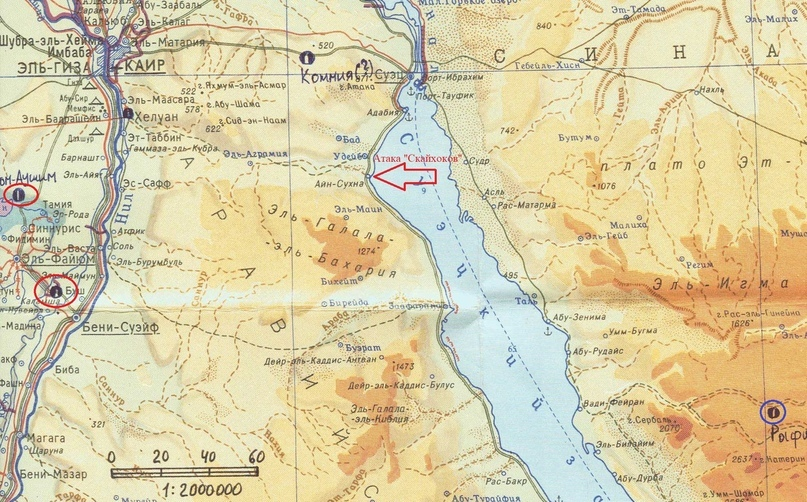
\includegraphics[scale=0.4]{Dolina_5/ZfWbBYQ2d98.jpg}
	%	\label{fig:scipion} % Unique label used for referencing the figure in-text\end{document}
	%	%\addcontentsline{toc}{figure}{Figure \ref{fig:placeholder}} % Uncomment to add the figure to the table of contents%----------------------------------------------------------------------------------------
	\caption{
		Карта (1) «Скайхоки» атакуют РЛС в районе Сохны. Отмечены основные аэродромы базирования советской авиации.}%	CHAPTER 2
\end{figure}

Для советской стороны это был ещё один день, такой же, как и все предыдущие. Израильтяне бомбили у Канала, а при появлении советских самолётов — уходили на Синай, прекрасно зная, что преследовать их не будут. Советские МиГ-и занимали привычную зону воздушного дежурства — между Сохненской и Заафранской долинами, южнее зоны ответственности ПВО. Израильтяне дожидались, пока у них закончится топливо - и бомбили снова. И так - ещё и ещё…

На севере (район Канала) была зона «ответственности» ПВО, советского и египетского. Но как только появлялись цели со стороны Суэцкого канала или залива — обе эскадрильи моментально переводились в готовность №1. Рубежом подъёма советских истребителей была зона «разграничения». Так и в этот раз: как только появились «цели», их сразу взяли на сопровождение. Как только они пересекали «красную черту», советские истребители поднимались в воздух. «Скайхоки», видимо, черту не пересекли.

\section{30 июля 1970 года, 14:20. Кот в мышеловке.}

ем временем, над Суэцким Заливом на малой высоте уже летит звено «Миражей». Они идут в плотном строю, словно их два, а не четыре, и действуют они, как пара самолётов фоторазведки.

Вспоминает Амос Амир (ведущий звена «разведчиков» и комэск и ас с 5 сбитыми МиГами в тот момент):

\begin{textcitation}
	В штабе ВВС и генштабе созрело мнение, что пора перестать избегать схваток с русскими МиГами ибо политика предоставления им неприкосновенности не оправдала себя. Раз русские начали вступать в прямое противоборство с израильской авиацией, надо начинать вести себя по-другому. Командиры пяти истребительных эскадрилий были приглашены в штаб ВВС, где их проинструктировал лично командующий ВВС.
	
	Я первым занял свою позицию для взлета. Затем, один за другим, подъехали и остальные машины моего звена. Ашер - Второй. Авраам - Третий. Гилад - Четвертый. До взлета оставалось несколько минут и я попытался подсчитать число побед, одержанных нашей четверкой. Получилось 20 побед на всех. Вряд ли, подумал я, где-либо ещё в мире есть звено с таким послужным списком.
	
	За 2 минуты до взлета я слегка отпустил РУД и самолет скользнул в позицию слева на полосе. Остальные тут же последовали за мной и заняли свои позиции. Мы быстро проверили работу двигателей. Было необходимо соблюдать радиомолчание как это обычно делалось при совершении дальних разведывательных полетов.
	
	Отнюдь не впервые, но с большей силой, чем обычно, я почувствовал волнение, распространяющееся по моим нервам и крови. То, что нам предстояло, было больше, чем охотой. Это не было преследованием пантерой смертельно испуганной лани. Это было состязанием со всеми картами на столе и ставками, выше которых не бывает. Нам предстоял смертельный бой, в котором всё позволено. Хитрость, трюки, изобретательность, знания, способность, личное мужество, сила - все эти качества скоро должны были подвергнуться суровому испытанию. Я знал точно, что требуется от нас, и хотя никогда ещё не встречался с русскими в бою, я был уверен в себе и своих товарищах. Наша задача была исключительно важна и как в прежние, более молодые годы, я почувствовал как пьянящее ощущение своей значимости разливается по всему телу.
	
	В назначенный момент, я дал “полный газ” двигателю, а затем включил форсаж и мой Мираж рванулся вперед. Остальные последовали за мной. Я повернул на запад и набрал высоту 35.000 футов (10,7 км), в направлении центрального Синая. Ашер, мой ведомый номер 2, расположился всего в нескольких метрах от меня. Левее его летел Авраам, Третий, в 700 метрах от меня. Гилад, Четвертый, его ведомый, также расположился очень близко к нему. На экране радара, оператор увидел бы только две отметки и решил бы, что летит одна пара, а не четверка.
	
	Я знал, что в эти же мгновения, другие звенья тоже готовятся к взлету. На авиабазе Рамат-Давид, Авиху возглавлял звено Фантомов, а за ним должно было следовать звено Миражей под командой Ури. Ещё одно звено Миражей во главе с Ифтахом готовилось на авиабазе Хатцор. Но никто не должен был ничего знать о них до критического момента. Им предстояло лететь к каналу на высоте верхушек деревьев.
\end{textcitation}

Насчет Хатцора, вероятно, Амоса подводит память — сам Спектор писал, что он стартовал с Рефидим.

\begin{figure}[h!tb] 
	\centering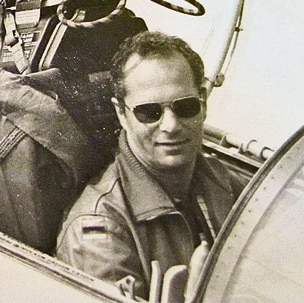
\includegraphics[scale=0.4]{Dolina_5/EbhtRCbIZCw.jpg}
	%	\label{fig:scipion} % Unique label used for referencing the figure in-text\end{document}
	%	%\addcontentsline{toc}{figure}{Figure \ref{fig:placeholder}} % Uncomment to add the figure to the table of contents%----------------------------------------------------------------------------------------
	\caption{Амос Амир (фото Ynet)}%	CHAPTER 2
\end{figure}

\textbf{Всё готово. Все действующие лица заняли свои позиции. «Приманка» появилась в небе Египта. Советские ВВС захватили наживку и бросились к ним.}

Вспоминает Амос Амир:

\begin{textcitation}
	Над центральным Синаем, в районе Джебел Либни, мы снизились и исчезли с экранов радаров. Мы пересекли Суэцкий залив и продолжили лететь на запад, углубляясь в египетскую территорию. Мне вдруг вспомнился мой первый полет над Египтом. С тех пор я участвовал в десятках глубоких рейдов над территорией противника и накопленный опыт безусловно сказывался. Напряжение присутствовало, но давящего страха не было.
	
	В намеченный момент я дал команду: “Красные, вперед!” Всё ещё двумя отдельными парами, на приличном расстоянии друг от друга, но по-прежнему летевшими в плотном строю, мы набрали высоту 35.000 футов (10,7 км), типичную для разведывательных полетов. Но у нас, конечно, не было фотокамер. Мы несли вместо них ракеты и снаряды, и были готовы нарушить нашу роль разведчиков в любой момент, вступив в воздушный бой.
\end{textcitation}

\textbf{А вот что в этой время происходило на советских аэродромах.}

Вспоминает полковник А.В. Акименков (в 1970м — замкомэска 1-й эскадрильи из Бени-Суэф, в дальнейшем — заслуженный лётчик-испытатель):

\begin{textcitation}
	Ближе к полудню 30 июля прозвучала команда «Воздух!» Но звенья повели не на север в сторону Суэцкого канала, а на юг, через запретную для полётов зону, закрытую ракетчиками. 
\end{textcitation}

В качестве «приманки» были «Миражи» 119-й эскадрильи. Почему именно они? Потому что именно 119-й принадлежали самолёты — разведчики, летавшие над Египтом раньше. И 119-й принадлежали пилоты этих машин, голоса которых отлично знали советские и египетские операторы. К тому-же, это звено было наиболее «заслуженным» из всех — на их счету в начале дня было 26 побед (!) У звена из 117-й их было 20.

\section{Что дальше:}

Вспоминает И.В. Рыболовлев - в 1970-м начальник группы объективного контроля Бени-Суэйф:

\begin{textcitation}
	После обеда воздушная обстановка была спокойная. <…> В 13:30-13:35 на экране РЛС появилась отметка, движущая на высоте 4500 метров из глубины территории противника со скоростью около 600 км/час, по характеристике цель была определена, как транспортный самолет. Подобные полеты транспортных самолетов проходили регулярно. В 13:45-13:50 южнее Суэц самолет развернулся на север и пошел вдоль линии фронта, на удалении 35-40 км. Через 10-12 минут, разворот на 180 градусов и т.д. Теперь эту цель классифицировали как воздушный пункт управления. В 14:05-14:10 штурман наведения ВПН Бир-Арейда доложил, что появились две группы самолетов в азимуте 50 градусов на удалении 120 км, следуют к каналу . Была дана команда дежурным звеньям 2-й и 3-й эскадрильям занять готовность 1, одновременно 2 аэ занять готовность 2. Через 3-4 минуты с арабского КП сообщили о неустойчивой проводке низко -летящей цели южнее Суэц на удалении 40 км от берега моря и арабы объявили на аэродроме воздушную тревогу.
\end{textcitation}

Отметим два момента. Во-первых, упоминания о «Скайхоках» отсутствуют — судя по всему, их просто посчитали не стоящей внимания целью. Во-вторых, до этого момента израильские и советские воспоминания полностью совпадают!

\begin{figure}[h!tb] 
	\centering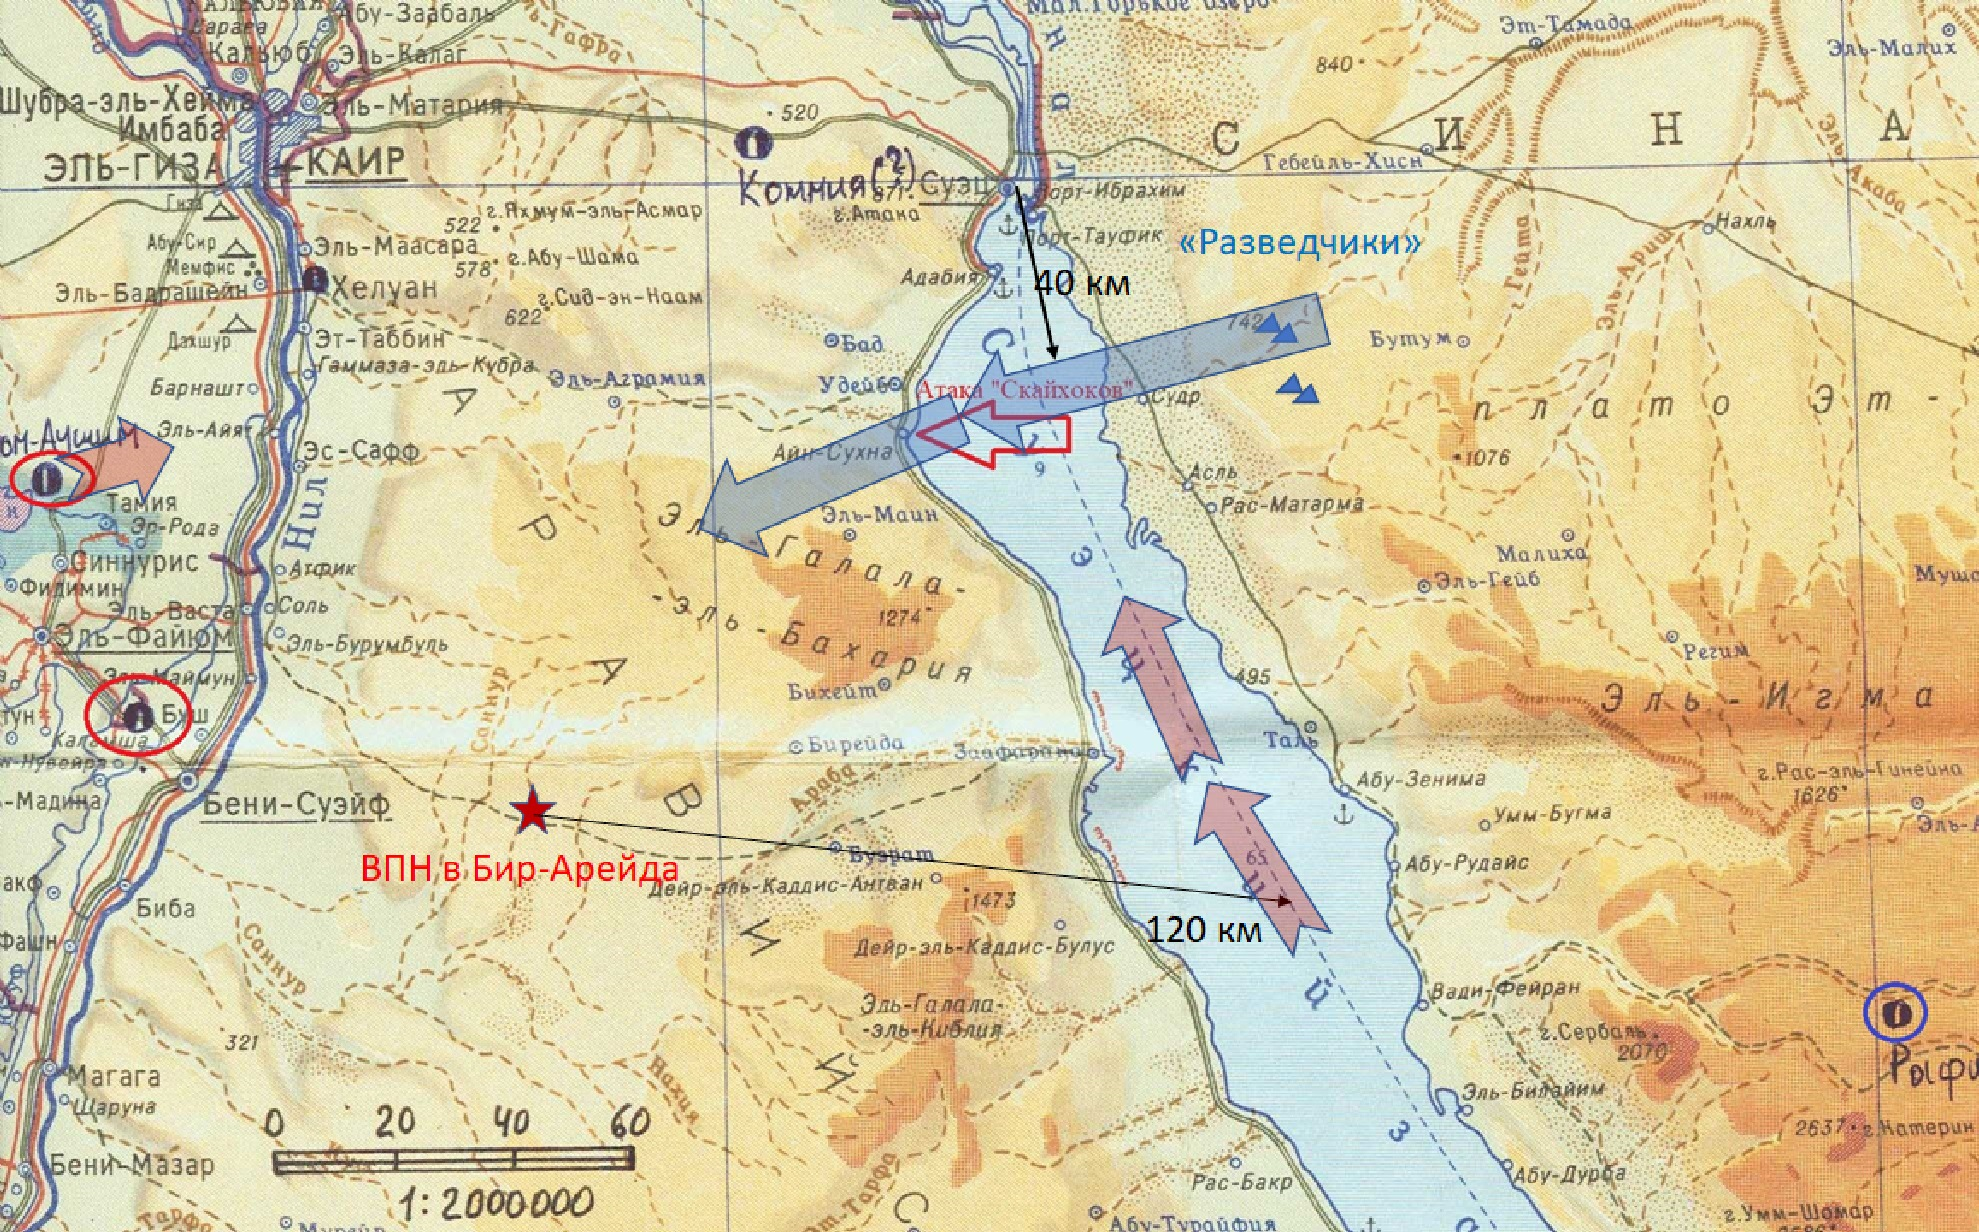
\includegraphics[scale=0.25]{Dolina_5/2p7rkGhu9Io.jpg}
	%	\label{fig:scipion} % Unique label used for referencing the figure in-text\end{document}
	%	%\addcontentsline{toc}{figure}{Figure \ref{fig:placeholder}} % Uncomment to add the figure to the table of contents%----------------------------------------------------------------------------------------
	\caption{Синий — предположительный маршрут «Разведчиков». Красный — проводка советским ВПН неизвестных самолётов (возможно, демонстративной группы). }%	CHAPTER 2
\end{figure}

Отметим, что обнаружить низколетящие «Миражи» звена Амоса Амира было для пункта наведения в Бир-Арейде достаточно затруднительно — между ними находился горный массив, да и расстояние (и как следствие — кривизна земли) особо не способствовали обнаружению. Египетские РЛС в Суэце — да, могли что-то заметить. Возможно, «Миражи» шли несколько южнее.

Продолжаем цитировать Рыболовлева:

\begin{textcitation}
	В 14:15 с ВПН доложили о появлении в воздухе над территорией противника вертолетов 5 км и 20 км севернее города Суец. Появление ВзПУ и вертолетов говорило о том, что противник готовится к выполнению операции (возможно, удар по переднему краю). Таких действий со стороны противника в нашей зоне давно не было. Майор Желтиков доложил на КП в Каир и предложил, после занятия готовности всей 2йэскадрильи поднять в воздух 10 самолетов (для занятия эскадрильей готовности 1 (из готовности 2, в которой она находилась - А.Н.) необходимо 10-12 минут. Перехват в составе десятки был отработан). Однако была дана команда поднять звено с аэродрома Комаушим и в случае необходимости на усиление звено с аэродрома Бени-Суэйф. Как стало известно позже, на КП в Каире в это время не работала РЛС, и они не видели обстановки в воздухе. 
	
	В 14:28 с аэродрома Комаушим взлетело звено под командованием Каменева, через 2-3 минуты с аэродрома Бени-Суэйф взлетело звено Юрченко. 
\end{textcitation}

«Появились две группы самолетов в азимуте 50 градусов на удалении 120 км, следуют к каналу,» — это и есть «Миражи» четвёрки «разведчиков» из воспоминаний Ашера Снира. Кто был «второй группой» самолётов - «Фантомы», другие «Миражи» или вторая пара звена Снира — неизвестно, да и не важно.

Смотрим воспоминания Бабича (советник в ВВС Сирии. В Египте он, насколько я знаю, практически не был, писал с чужих слов и допускал множество ошибок, однако в его работах есть очень любопытные подробности, известные явно со слов человека, бывшего на месте):

\begin{textcitation}
	15:20 РЛС ПВО Египта засекла на 4000 4 «Скайхока», шедших на запад. Одновременно были обнаружены 2 пары «Фантомов»,которые на 7000 шли со скоростью 800 курсом 350 вдоль побережья Красного моря. В 15:28 и 15:30 с двух египетских аэродромов подняты 2 звена МиГ-21 пилотируемые советскими лётчиками. Поскольку противник вёл себя неактивно, их вывели на 8000 в зоны дежурства. В 15:34, описав широкую дугу северо-восточнее Сухны (западное побережье Красного моря) Скайхоки со снижением повернули обратно и вышли из зоны РЛС Египта. МиГи остались патрулировать в зонах.
\end{textcitation}

\textbf{Судя по всему, «Скайхоки» — это на самом деле «Миражи». }

Дальше, мне кажется, слишком много противоречий с существующими советскими и израильскими воспоминаниями. Но общий смысл — перехватчики подняли, «Миражи» начали уходить за Канал — перехватчики вывели в зоны дежурства — неизменен.

Итак, к этому моменту советские и израильские воспоминания сходятся с поразительной точностью. За исключением одного момента — об израильских самолётах над Заливом сообщили в 14:15. Звено Каменева поднялось в воздух в 14:30. Что израильтяне делали всё это время?

Отвечает Амос Амир:

\begin{textcitation}
	Мы уже приближались к долине Нила, когда мы повернули вправо и полетели в северо-восточном направлении. Глянув влево сквозь мерцающее марево горячего, влажного воздуха, я увидел зеленую ленту долины Нила, протянувшуюся с севера на юг.
	
	Красные, включить фотокамеры! - отдал я приказ чтобы запутать египетскую разведку. Мы продолжали лететь в направлении города Суэц.
	
	Красные, это Золотой. Огурец! - пришло сообщение из командного центра.
	
	Это Красный. Вас понял - ответил я. Красные, поворачиваем влево. Мы опять стали углубляться в территорию Египта. Я знал, что этот наш маневр будет слишком соблазнительным для египтян и они заглотят наживку. Они просто обязаны будут послать перехватчики против этих двух нахальных израильских воздушных шпионов. И мы надеялись, конечно, что на перехват вылетят русские. У нас были все основания надеяться на это, но точно узнать мы могли только через некоторое время после боя.
\end{textcitation}

Так вот, ответ — минут 5-10 они то углублялись на территорию Египта, то возвращались назад к Каналу. А на советских аэродромах в это время быстро поднимали в воздух истребители. Здесь нет никакой мистики. 

\begin{figure}[h!tb] 
	\centering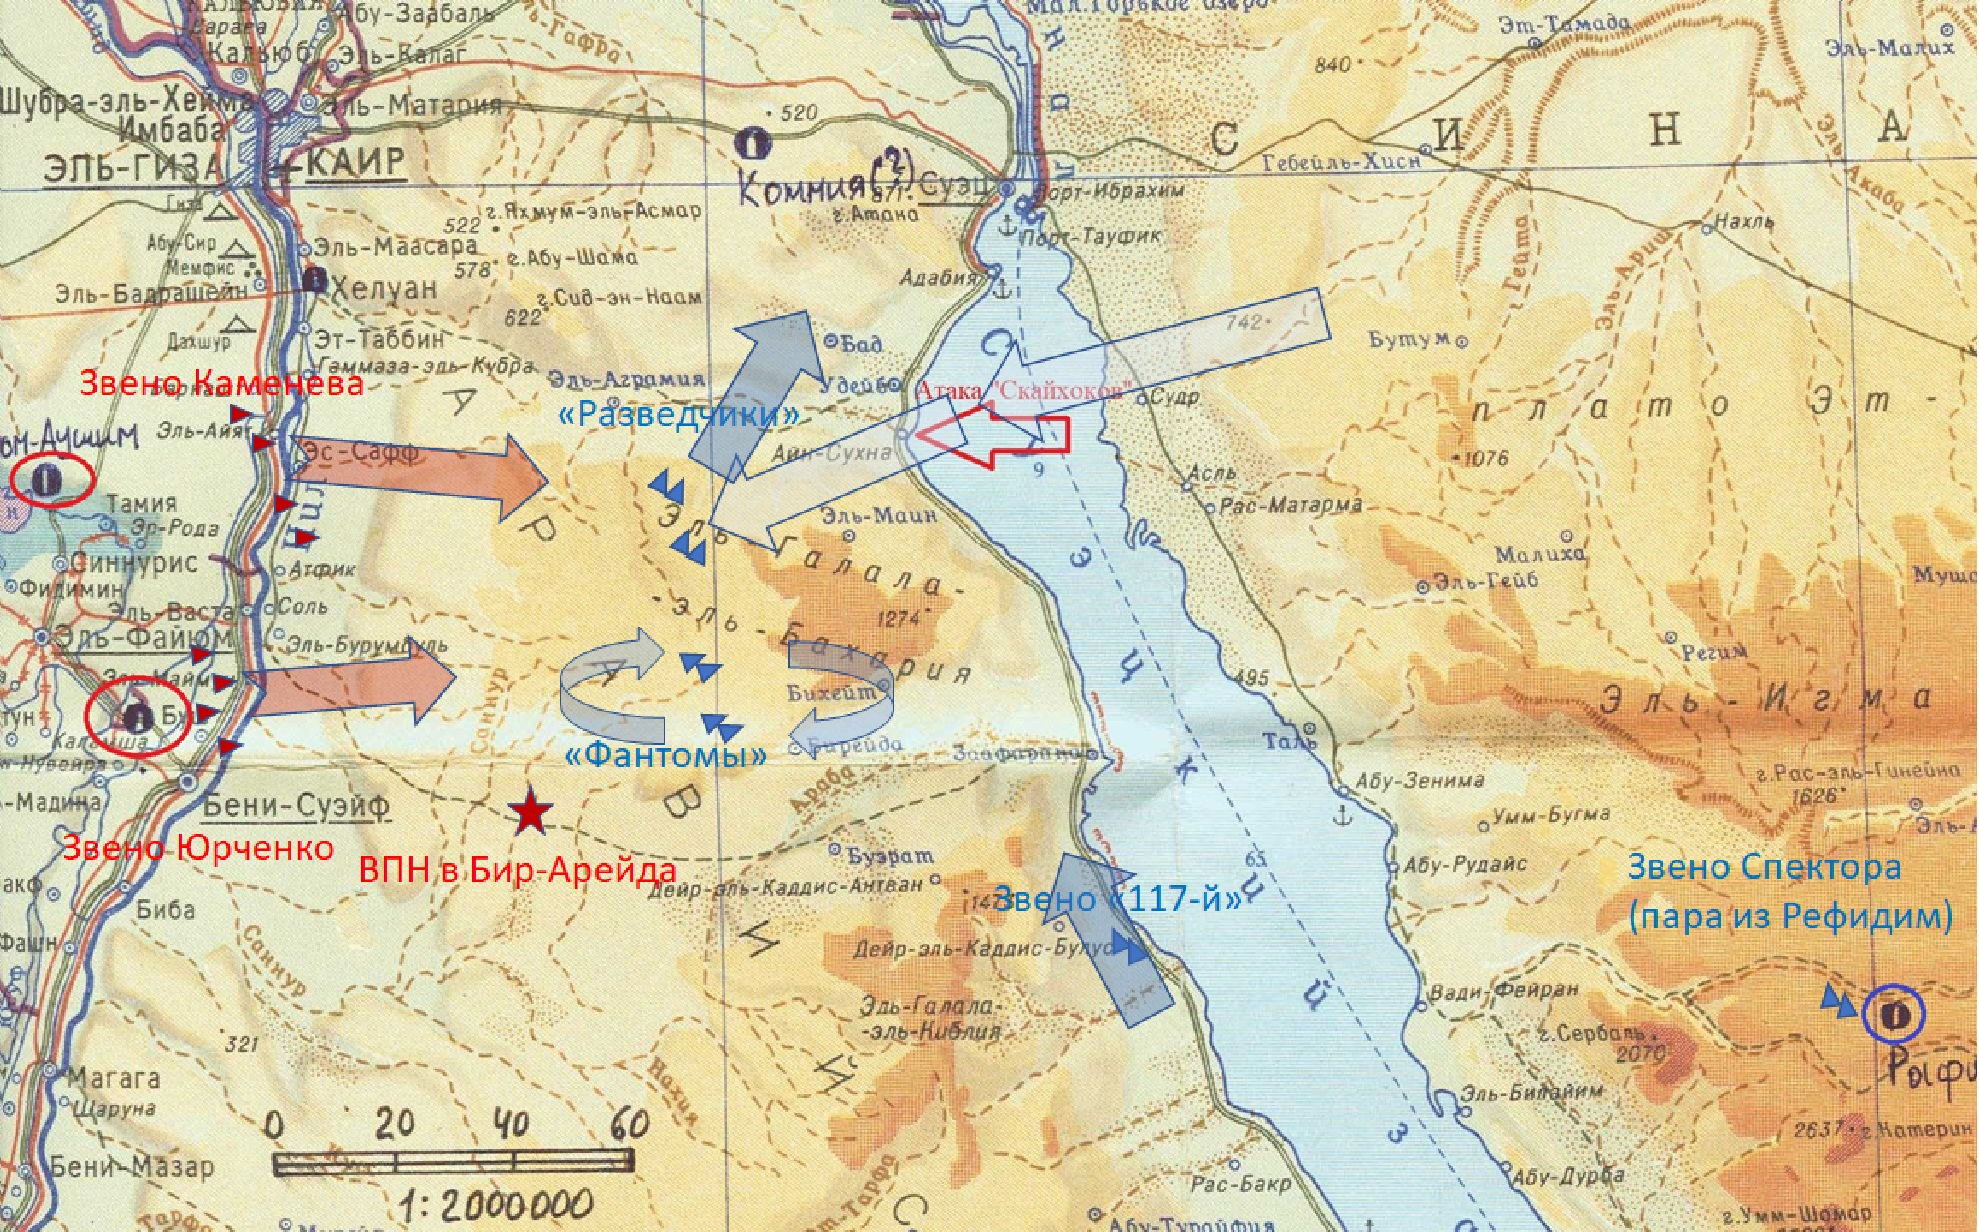
\includegraphics[scale=0.25]{Dolina_5/ozXWHNIA4io.jpg}
	%	\label{fig:scipion} % Unique label used for referencing the figure in-text\end{document}
	%	%\addcontentsline{toc}{figure}{Figure \ref{fig:placeholder}} % Uncomment to add the figure to the table of contents%----------------------------------------------------------------------------------------
	\caption{Советские самолёты поднимаются на перехват. Первым — звено Камнева, вторым — Юрченко. «Разведчики» маневрируют в зоне западнее Залива. }%	CHAPTER 2
\end{figure}

Примерно то-же самое мы видим в другой израильской статье — Рапопорта в «Маариве» 

\begin{textcitation}
	У русских ушло 11 минут, чтобы наконец решиться поднять самолёты.
\end{textcitation}

Снова Амир:

\begin{textcitation}
	Красные, это Золотой! Помидор! - пришло новое сообщение с КП. Это означало, что египтяне клюнули. Кодовое слово означало, что к нам приближаются самолеты противника.
	
	Красные, разворачиваемся. Сбросить баки - скомандовал я. Мы развернулись на восток, чтобы бой прошел поближе к нашей территории. Теперь, когда наше подбрюшье освободилось от тяжести подвесных баков, «Миражи» опять обрели свою обычную резвость и мы быстро ускорялись. По моей команде, мы все ещё раз проверили все наши системы и оружие. Через несколько секунд этот маскарад закончится, перчатки будут сброшены и небо озарится огнем!
\end{textcitation}
Мне кажется (и это больше соответствует логике дальнейших событий), что баки они сбросили не перед, а после того, как развернулись. Скорее даже после того, как повернули обратно и начали сближение. В любом случае, здесь главное — «развернулись на восток». Не позднее 14:30 израильтяне заметили устремившиеся к ним две четвёрки советских истребителей.

Смотрим воспоминания Авраама Салмона из книги Дани Шалома «Призраки над Каиром»:

\begin{textcitation}
	Авраам Салмон [первое" звено "Миражей", 119 эскадрилья]: "МиГи шли с запада, и мы в определенный момент повернули на восток, когда до них было 10-15 миль, чтобы увлечь их за собой на восток…
\end{textcitation}

Смотрим на воспоминания Рыболовлева:

\begin{textcitation}
	При приближение звена Каменева на расстояние 40-50 км, группа израильских самолетов развернулась и, перелетев канал, заняла зону. С ВПН Бир-Арейда дали команду звену Каменева занять зону (не помню номер, северную), а звену Юрченко следовать в южную зону. Израильтяне ждали, когда звено Юрченко займет зону и решали задачу, что делать со звеном в северной зоне.
\end{textcitation}

\begin{figure}[h!tb] 
	\centering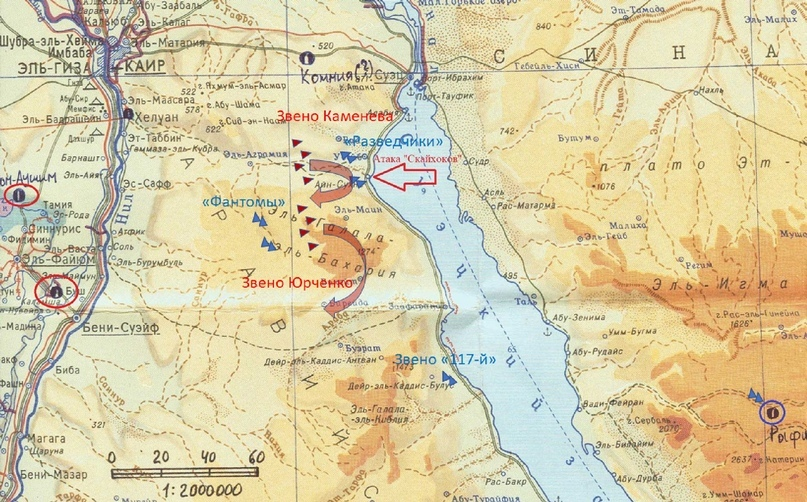
\includegraphics[scale=0.25]{Dolina_5/L5R5y0f-QOA.jpg}
	%	\label{fig:scipion} % Unique label used for referencing the figure in-text\end{document}
	%	%\addcontentsline{toc}{figure}{Figure \ref{fig:placeholder}} % Uncomment to add the figure to the table of contents%----------------------------------------------------------------------------------------
	\caption{Приблизительно в 15:35 советские самолёты подходят к месту нахождения израильских «разведчиков» — звено Каменева первым, звено Юрченко — вторым. Израильтяне уходят к Каналу, советские самолёты занимают установленные зоны дежурства, северную и южную. }%	CHAPTER 2
\end{figure}

В итоге — что мы видим? Советские МиГи не преследуют (!) уходящие «Миражи», это бесперспективно. Израильтяне десятки раз уходили за Канал — уйдут и снова. Советские пилоты занимают установленные зоны дежурства в воздухе. В это время, видимо, срывается израильский план, по которому их должны были атаковать с малой высоты «Фантомы» — происходит нестыковка по времени. Или, что прозаичнее, банальное недопонимание.

Примерно в то же время у израильтян случается ещё одна накладка: одна из пар второго звена «Миражей» (звено «Эвена») обнаруживает проблему с двигателем у ведущего и возвращается домой. Теперь на усилении у израильтян всего два «Миража», плюс четвёрка в Рефидим, которая всё ещё на земле. Четыре «Миража» и четыре «Фантома» на малой высоте против восьми МиГ-21. Маловато для «огромного численного превосходства», столь часто описываемого в советских источниках.

Делаем промежуточные выводы:

\begin{itemize}
	\item Большую часть пути звено «разведчиков» прошло на малой высоте, показавшись на экранах радаров лишь в глубине Египта приблизительно в 14:20.
	\item Советские и египетские РЛС видят «разведчиков», не видят другие израильские самолёты, и реагируют соответствующе — поднимают в воздух всего 8 МиГ-21 вместо потенциальных 10-20.
	\item Советское командование не имеет представления о реальной сути происходящего и действует так же, как и в предыдущие дни, предполагая, что израильтяне снова будут избегать боя.
	\item Между советской и израильской версиями минимум противоречий
\end{itemize}



\section{30 июля 1970 года, 14:40. Сближение.}

Итак, диспозиция: два советских звена в воздухе, израильтяне где-то восточнее.

Израильтяне доворачивают на запад. Маски сброшены — из пары безоружных самолётов фоторазведки они превращаются обратно в одну из лучших истребительных четвёрок Израиля.

Амос Амир:

\begin{textcitation}
	Красные, это Золотой. Атакуйте, азимут два, пять, ноль. Четверка противника впереди вас в 20 милях (35 км) и ещё одна позади них, в 35 милях (55 км).
	
	Вас понял. Начинаем перец. Я скомандовал включить форсаж. На запасной частоте я начал слышать голоса командиров двух других наших звеньев, в которых я узнал Авиху и Ифтаха.
	
	Красный, выше на 11 часах - в моих наушниках раздался голос Авраама. И я тут же увидел пару МиГов, пролетавших высоко над нами в противоположном направлении.
	
	Третий, атакуй южную пару, а мы займемся северной, той что повыше. Авраам, мой Третий, тут же подтвердил получение команды.
	
	Красные, это Золотой. Внимание, вторая четверка приближается к району боя. А через две с половиной минуты в бой вступит третья четверка - известил КП всех наших в воздухе.
\end{textcitation}


«Третья четвёрка» — это третье советское звено, Саранина. То есть, по воспоминаниям израильтян, они оказались в воздухе ДО начала боя.

К слову о «начинаем перец». «Перец», «Пеппер» — классическое израильское название для форсажного режима работы двигателя. Воюют на форсаже, так что «начинаем перец» — включаем форсаж, входим в бой.

Авиху (Бен-Нун) был достаточно близко — а Спектор в тот момент только стартовал.

Как видели это с советской стороны?

Бабич:

\begin{textcitation}
	В 15:37 в небе появились новые цели 3-го звена Миражей в сомкнутом боевом строю на 7000 (высоты - А.Н.)со скоростью около 1000 шли севернее Сухны в направлении северной зоны дежурства. МиГов тут же развернули навстречу противнику по командам с земли.
\end{textcitation}

Ну, «три звена «Миражей» — это явный перебор, тут у страха глаза велики. Не знаю, что сыграло роль — желание объяснить поражение огромным численным превосходством противника или неразбериха. Фактически, максимум — это превращение пары в четвёрку. Кстати, по воспоминаниям других участников, советский КП звено Амоса Амира изначально идентифицировал как четвёрку. Тут есть некоторое противоречие между советскими воспоминаниями — это вполне нормально.

\begin{figure}[h!tb] 
	\centering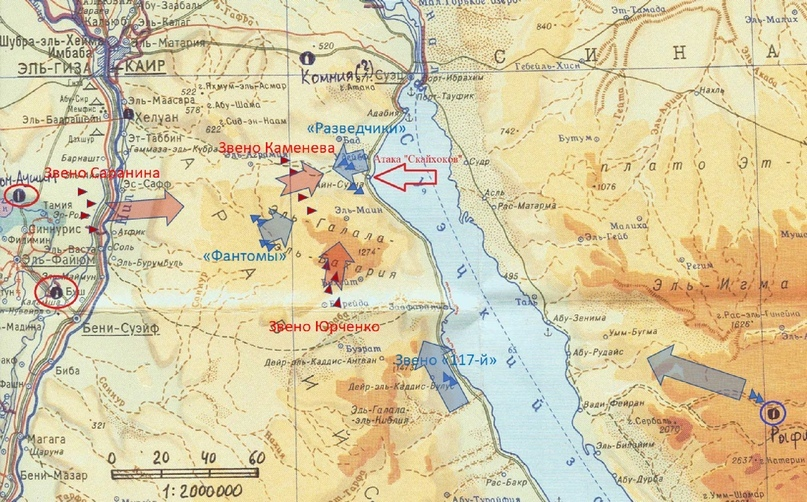
\includegraphics[scale=0.25]{Dolina_5/hqH_3szaow8.jpg}
	%	\label{fig:scipion} % Unique label used for referencing the figure in-text\end{document}
	%	%\addcontentsline{toc}{figure}{Figure \ref{fig:placeholder}} % Uncomment to add the figure to the table of contents%----------------------------------------------------------------------------------------
	\caption{Сближение. Первыми под удар «Миражей» попало звено Камнева. Из Рефидим взлетает Спектор и Цук. Корен-Рихтер из 117-й на форсаже летят к месту боя. «Фантомы» набирают высоту. В Ком-Аушим спешно поднимают третье звено. }%	CHAPTER 2
\end{figure}

Примерно в то же время оставшаяся пара 117-й выдвигается в бой. С Рефидим стартует пара Йифтаха Спектора (чуть позже его ведомый, Михаэль Цук, потеряет Спектора и вернётся домой).

Кстати, про «огромное численное превосходство». Есть ещё одна интересная гипотеза, высказанная капитаном ВВС Израиля Максимом на форуме «авиабазы». По его словам, в израильских отчётах о том бое описывается, что советские лётчики, возможно, приняли сброшенные топливные баки за другие «Миражи», к немалому удивлению израильтян — такой «фокус» не был запланирован. По идее, этим можно объяснить уверенно описываемое почти всеми советскими источниками огромное израильское численное превосходство. Можно ли принять топливный бак за самолёт? Он по длине меньше где-то в 2,5 раза. Не знаю. Но гипотеза такая существует.

\begin{figure}[h!tb] 
	\centering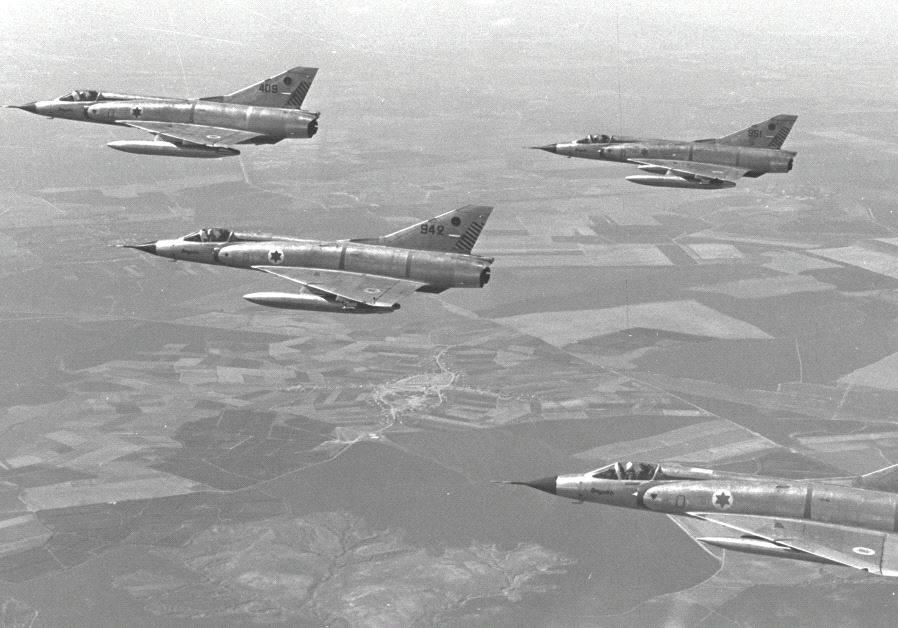
\includegraphics[scale=0.25]{Dolina_5/E47r1x-NUmM.jpg}
	%	\label{fig:scipion} % Unique label used for referencing the figure in-text\end{document}
	%	%\addcontentsline{toc}{figure}{Figure \ref{fig:placeholder}} % Uncomment to add the figure to the table of contents%----------------------------------------------------------------------------------------
	\caption{Строй «Миражей», топливные баки под крыльями.}%	CHAPTER 2
\end{figure}

Рыболовлев:

\begin{textcitation}
	Как только звено Юрченко заняло зону, израильская группа (4 или 8 самолетов) из зоны перешла канал и взяла курс на звено Юрченко. Штурман ВПН Бир-Арейда дал команду на перехват звену Каменева (звено находилось ближе к противнику на 25-30 км, чем звено Юрченко), уточнил данные о противнике, одновременно дана была команда на перехват звену Юрченко. По команде на перехват, летчики сбрасывают подвесные топливные баки и включают форсаж. (Высказывание некоторых израильских летчиков об опасности столкнуться со сброшенными топливными баками байки. Топливные баки были сброшены за 30 км до встречи).
\end{textcitation}

Здесь тоже небольшая ошибка — целью израильтян было именно «северное» звено Каменева. Насчет «высказываний об опасности столкнуться» — да, сброшены они были сильно до встречи — но так и «жалуются» на них не пилоты «Миражей», а пилоты «Фантомов» (конкретно Села), которые в тот момент были на малой высоте, в нескольких километрах ниже советских МиГов.

\section{30 июля 1970 года, 14:42. Огонь в небесах.}

Ельчанинов:

\begin{textcitation}
	Капитан Юрченко доложил на командный пункт: «Вижу четвёрку истребителей».
\end{textcitation}

Что характерно — никаких «десятков» «Миражей». Четвёрку.

Амос Амир:

\begin{textcitation}
	Красный, выше на 11 часах - в моих наушниках раздался голос Авраама (Салмона, ведущего второй пары). И я тут же увидел пару МиГов, пролетавших высоко над нами в противоположном направлении.
	
	Третий, атакуй южную пару, а мы займемся северной, той что повыше. Авраам, мой Третий, тут же подтвердил получение команды.
	
	Красные, это Золотой. Внимание, вторая четверка приближается к району боя. А через две с половиной минуты в бой вступит третья четверка - известил КП всех наших в воздухе.
	
	В резком вертикальном маневре задрав нос своей машины, я направился навстречу двум МиГам, пикировавшим на нас с высоты. Слепящий свет в лицо не дал мне возможности продолжать следить за МиГами, и вдруг я услышал голос Ашера, Второго и моего ведомого: МиГ проскочил мимо меня слева. Я атакую его.
	
	Мне это не очень понравилось, так как это означало, что моя пара разбивалась на два одиночных истребителя без взаимной поддержки. Я глянул влево, но не увидел ни Миража, ни МиГа.
\end{textcitation}

«Вторая четвёрка» — это звено Юрченко. Третья — звено Саранина.

\begin{figure}[h!tb] 
	\centering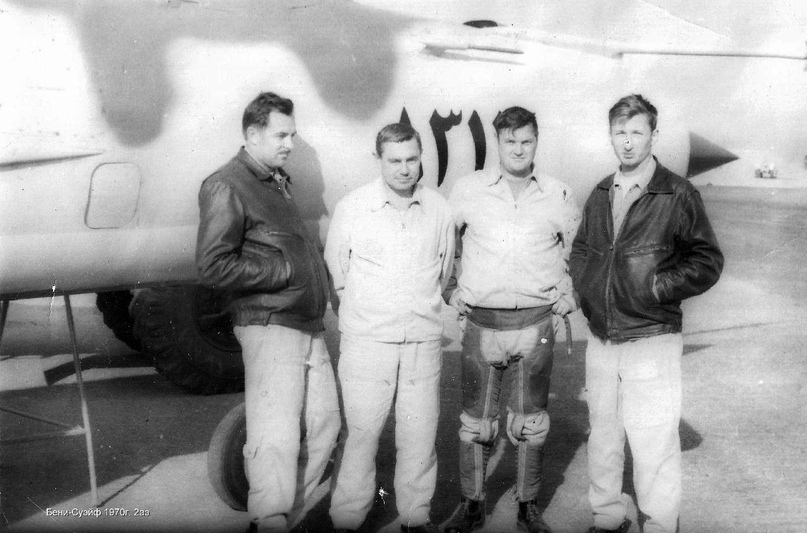
\includegraphics[scale=0.25]{Dolina_5/jnKCAz-mYKE.jpg}
	%	\label{fig:scipion} % Unique label used for referencing the figure in-text\end{document}
	%	%\addcontentsline{toc}{figure}{Figure \ref{fig:placeholder}} % Uncomment to add the figure to the table of contents%----------------------------------------------------------------------------------------
	\caption{Дежурное звено Саранина, Слева направо: В.А. Махоткин, В.Ф. Васильев, В.Ф. Саранин, В.И. Рыжов МиГ-21 (бортовой №831... (8311, 8312, 8313 ?)). 135 иап. Ком-Аушим. (из личного архива В.Ф. Васильева). Фото с сайта hubara-rus}%	CHAPTER 2
\end{figure}

К сожалению, воспоминаний о начале боя с советской стороны практически нет — мы даже фамилий всех лётчиков не знаем. По одной из версий, ими были капитаны Рахманкин и Хтей.

В то же время, к месту боя на всех парах движется четвёрка Ифтаха Спектора — собственно, пара «Миражей» Спектора из Рефидим и пара Гиоры Фурмана из Хацора.

Дани Шалом (перевод Наума Шубаева):

\begin{textcitation}
	Майор Йифтах Спектор, командир первой истребительной [101] эскадрильи, уже стоял на краю [взлетной] полосы, с включенным двигателем, когда получил приказ вступить в бой. Все это время он слушал, в нетерпеливом ожидании, [следя за тем, что] происходило в небе Египта, и ему не нужно было повторять дважды. <...>
\end{textcitation}

Начался бой. Дальше карты рисовать бессмысленно: слишком много динамики и слишком мало известных географических ориентиров. Обстановка постоянно менялась, и её сложно формализовать на картинке.

К сожалению, если израильские пилоты оставили подробнейшие описания всего происходящего (Ашер Снир от пилотов «Миражей», Авиху Бен-Нун и Авием Села от «Фантомов»), то воспоминания советских лётчиков, если и существуют в природе, то практически недоступны. Причин тут две. Первая — параноидальная секретность того времени. Вторая причина гораздо банальнее — из восьми участников боя трое погибли, трое вышли из него достаточно быстро. Оставшиеся двое (Сыркин и Макара) не оставили ничего, кроме двух предложений в статье Заборского. Повторюсь, мы даже не знаем имён всех из них..

В итоге самые «близкие» к месту событий люди, оставившие хоть какую-то информацию — это лётчики Васильев (звено Саранина) и Ельчанинов (был в Бени-Суэф в то время) плюс Рыболовлев.

Поэтому дальнейшие события будут строиться в первую очередь со слов израильтян, и по возможности — верифицироваться советской стороной.

Итак. Четвёрка «Миражей» атакует звено Каменева. У «Миражей» больший запас топлива — они благополучно летели на экономном режиме, в то время, как МиГ-и большую часть времени шли на форсаже. МиГ-21 может вести бой на форсаже порядка шести минут — после этого у него закончится топливо, что, в общем, и случилось.

Приблизительно в это время, в бой вступает ещё одна сила — израильское подразделение РЭБ и разведки, «Гречки» Тувьи Фейнмана и Аарона Ярива. Связь советских лётчиков в КП практически пропадает, а вместо чётких команд они слышат какие-то непонятные приказы. И тут же — эфир бьёт им по барабанным перепонкам. Роль «гречкоим» сложно оценить — но на следующий день пилоты отправили им корзину шампанского в качестве признания заслуг.

В первые же секунды бой распался на несколько одиночных.

Амос Амир:

\begin{textcitation}
	В резком вертикальном маневре задрав нос своей машины, я направился навстречу двум МиГам, пикировавшим на нас с высоты. Слепящий свет в лицо не дал мне возможности продолжать следить за МиГами, и вдруг я услышал голос Ашера, Второго и моего ведомого: МиГ проскочил мимо меня слева. Я атакую его.
	
	Мне это не очень понравилось, так как это означало, что моя пара разбивалась на два одиночных истребителя без взаимной поддержки. Я глянул влево, но не увидел, ни Миража, ни МиГа.
	
	В этот момент в эфире прозвучал голос Авраама: Это Третий. Я только что сбил одного из них. На запасной частоте я слышал голоса наших партнеров на Миражах и Фантомах, которые уже тоже находились в гуще боя.
\end{textcitation}

В тот момент, в бой уже вступили «Фантомы» и вторая четвёрка МиГ-21 (Юрченко). Авраам Салмон сбивает первый МиГ-21. 

\begin{figure}[h!tb] 
	\centering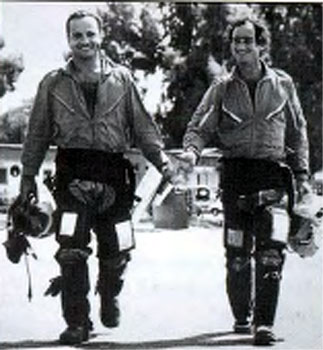
\includegraphics[scale=0.25]{Dolina_5/NX7h3zem5P0.jpg}
	%	\label{fig:scipion} % Unique label used for referencing the figure in-text\end{document}
	%	%\addcontentsline{toc}{figure}{Figure \ref{fig:placeholder}} % Uncomment to add the figure to the table of contents%----------------------------------------------------------------------------------------
	\caption{Авраам Салмон (слева)}%	CHAPTER 2
\end{figure}

Кто это мог быть?

Авраам Салмон (по книге Дани Шалома):

\begin{textcitation}
	Мой ведомый ушел в сторону, а я увидел МиГ и откинул "ложечку" [- предохранитель гашетки], однако он выглядел не совсем как МиГ, поэтому я не произвел пуск". Это действительно был "Фантом" и тут я увидел позади него пару МиГов". Аврамик вышел в эфир и предупредил своих товарищей: "Осторожно, 'Кувалды'" Немного взволнованный, Аврамик обрадовался своему самообладанию. Он предупредил Авигу, повернул налево и выровнялся позади ведомого МиГа. Тот был слишком далеко, тем не менее выпустил ракету AIM-9D Саиндуиндер, которая поразила самолет. МиГ дернулся, поднял нос и вдруг взорвался. Салмон увидел парашют.
	
	Это был капитан Николай Юрченко, командир эскадрильи из Бени-Суэйфа. Русский МиГ был поврежден, задымил, стал снижаться и ушел на запад.
	
	Пилот, который пытался выпрыгнуть с парашютом, погиб.
\end{textcitation}

Первая ошибка. Итак. Мы точно знаем, что Юрченко единственный из троих погибших не успел катапультироваться — его самолёт буквально взорвался в воздухе несколькими минутами позже.

Ельчанинов:

\begin{textcitation}
	Самолет же Юрченко подвергся прямому попаданию ракеты. Самолет взорвался, летчик погиб.
\end{textcitation}

Всё верно, только Юрченко погиб последним. Может быть, это был Журавлёв? Что мы знаем о его гибели?

Рыболовлев (лётчик звена Саранина, из поста на forumavia):

\begin{textcitation}
	из звена Камнева на аэродром не вернулся Журавлев, как его сбили и, что с ним случилось, никто не видел, остальные невредимые совершили посадку. Так доложили на КП полка, после посадки. Если я не ошибаюсь, в это время еще не на всех самолетах имелись перископы заднего вида.
\end{textcitation}
Васильев:

\begin{textcitation}
	После размыкания «Миражей», не смотря на большое превосходство противника (не менее 12-ти самолетов), четверка Каменева была введена в бой. Бой происходил на вертикальном маневре на высотах 2000-6000м. Журавлев – крайний ведомый был сбит и катапультировался.
\end{textcitation}

Акименков:

\begin{textcitation}
	По остатку топлива 1 300 кг и разрешающей команде полкового КП звено вышло из боя с пикированием к земле и разгоном предельной скорости, т.е. спасло себя.
	
	К сожалению, один из пилотов оказался без противоперегрузочного костюма, во время маневра из-за «чёрной пелены» в глазах потерял своих коллег, уменьшил перегрузку и тут же был сбит.
\end{textcitation}

Похоже, это действительно был Журавлев. Он сумел успешно катапультировался, но погиб при приземлении.

Итак. Что мы узнали?

В начале боя, четвёрка МиГ-21 лоб в лоб столкнулась с четвёркой «Миражей». Тот факт, что вместо пары невооруженных разведчиков они оказались четвёркой истребителей — неприятный сюрприз, но на «засаду» не тянет. Практически сразу бой принял хаотичный характер — в него вступили «Фантомы» и вторая четвёрка МиГ-21. При этом «Миражи» практически сразу «разбили пары» и вели бой в одиночку.

«Фантомы» практически не смогли реализовать своё преимущество внезапности — более того, прежде чем кого-то сбить, они ввязались в ближний манёвренный бой и достаточно долго в нём крутились. Очень быстро преимущество внезапности улетучилось, теперь это был просто большой воздушный бой.

Первую победу одержал Авраам Салмон — он атаковал самолёт выходившего из боя капитана Журавлёва, и сбил его. Продолжаем. В бой вступают «Фантомы» 69-й эскадрильи.

\begin{figure}[h!tb] 
	\centering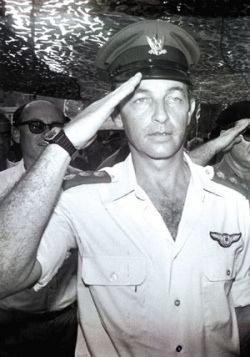
\includegraphics[scale=0.25]{Dolina_5/eUWubHXS7UA.jpg}
	%	\label{fig:scipion} % Unique label used for referencing the figure in-text\end{document}
	%	%\addcontentsline{toc}{figure}{Figure \ref{fig:placeholder}} % Uncomment to add the figure to the table of contents%----------------------------------------------------------------------------------------
	\caption{Авием Села}%	CHAPTER 2
\end{figure}

Авием Села:

\begin{textcitation}
	Они шли на нас парами, а мы дали им всем проскочить, чтобы не дать им взять нас в клещи, как они планировали. Они промчались мимо нас, пара за парой, как на параде. Мы подождали и направились за ними, зажимая их между собой.
\end{textcitation}

Амос Амир:

\begin{textcitation}
	Большая тень самолета промелькнула над моей кабиной. Я посчитал, что это был МиГ. Я очень быстро заложил вираж в направлении пикировавшего МиГа. Невдалеке от меня к югу, я увидел два грибовидных облака дыма, поднимающихся кверху от двух горящих МиГов.
	
	Это Второй, я сбил одного! - прозвучал голос Ашера. А я подумал про себя: И черт тебя знает, где ты сейчас находишься.
\end{textcitation}

Здесь есть определённое противоречие — Амос говорит о двух грибовидных облаках. Спишем это на подводящую память и годы.

Дани Шалом:

\begin{textcitation}
	Ашер Снир стал вторым пилотом, одержавшим воздушную победу. Он был ведомым А.Амира. На высоте 30 тыс футов (10 тыс. м) заметил русский МиГ, пошел на сближение с ним и сообщил Амиру: "Слева от меня прошел МиГ, преследую его". Амира это удивило - ведомый должен защищать ведущего и оставаться рядом.
	
	Снир был напорист и действовал быстро. Он осмотрелся: четыре МиГа и два "Фантома" были поблизости. Он повернул влево, в сторону одного из МиГов, который изо всех сил старался забраться выше, но скорость его была мала для такого маневра, и вскоре он потерял потенциал. Прицельная система работала исправно: головка самонаведения ракеты AIM-9D (Дэкер) засекла тепло МиГа - громкий сигнал зуммера - и Снир выпустил ее нажатием на гашетку. Ракета ушла вверх, воткнулась в брюхо МиГа и взорвала его. 
\end{textcitation}

Скорее всего, это МиГ-21 Яковлева или Сыркина.

Сыркин (по статье Заборского):

\begin{textcitation}
	Когда мы сблизились по наведению с групповой целью, - рассказывал он, - она вдруг рассыпалась, и перед нами почти в строю фронта как бы облавой оказалось больше десятка - не успел сосчитать - самолетов. Опознал их визуально как 'Миражи'. Передаю ведомому: 'Атакуем третью слева пару'. Начал маневрирование. Вдруг слышу от ведомого: 'Осторожно! Внизу 'Фантомы'! Ракеты!'. Начал противоракетный маневр - вдруг удар, и я кувыркаюсь. В хвосте, видимо, ракета. Катапультировался. 
\end{textcitation}

Акименков:

\begin{textcitation}
	Мимо наших ребят слева направо пронёсся «Мираж», который находился в левом развороте. Командир звена вводит самолёт в правый разворот и почти сразу же перекладывает его в левый крен, пытаясь выстроить кривую прицеливания для пуска ракет.
	
	В это время его ведомый видит в перископ пуск ракеты вторым «Миражом» и кричит о пуске командиру, выполняя одновременно размазанную «кадушку» и сбивая захват своего самолёта головкой самонаведения вражеской ракеты. Командир медлит с «кадушкой», поскольку его собственные ракеты уже захватили тепло летящего впереди противника.
	
	Далее - взрыв. От командира остался только пистолет. Всё остальное в аэрозольном состоянии стало принадлежностью долины.
\end{textcitation}


Про «командира» — это явная ошибка. Юрченко, командир звена, действительно погиб во взорвавшемся самолёте, но значительно позже и при других обстоятельствах. По его ведомому (Макара) действительно было несколько пусков ракет, но мне кажется, что в описании Акименкова всё же смешались два разнесённых по месту и времени эпизода.

Снова Акименков:

\begin{textcitation}
	Судьба второй пары была более простой, но не менее трагичной. На развороте звена вправо снизу сзади и мимо крайнего ведомого проскакивает «Фантом», но звено перекладывает крен влево и ведомый не успевает отстреляться, выдерживая место в боевом порядке. Естественно, кричит, что «Фантомы» сзади, и через мгновение получает ракету в двигатель. Самолёт переворачивает взрывом и лётчик в таком положении катапультируется, повреждая себе позвоночник. В последующем долго лечится, но остаётся в строю и делает успешную служебную карьеру.
\end{textcitation}


Это уже почти совпадает с другими описаниями! И манёвренный бой с «Фантомами», и предупреждение ведомого Сыркина, Яковлева: «Фантомы внизу!»

Здесь сложно что-то утверждать наверняка — но больше похоже на то, что Снир сбил именно Сыркина. Вопреки распространённому в советских источниках мнению, он не попал под атаку «Фантомов» снизу-вверх, а был сбит «Миражем» в манёвренном бою. «Фантомы» были рядом, но скорее всего просто пока проигрывали и МиГ-21, и «Миражам» по энергетике: всё же они набирали высоту, а не теряли её, разменивая на манёвр.

Здесь начинается одна из самых загадочных историй того дня. Дело в том, что через несколько секунд после успешной атаки, «Мираж» Ашера Снира был подбит сам. Кем? Это самое интересное.

В 90-х годах в итальянской газете появилось интервью от имени некоего генерала Владимира Ивлева, который, якобы, был участником того боя, и даже сбил один «Мираж».

Приводятся его слова (по книге Дани Шалома):

\begin{textcitation}
	"Мое сердце начало сильно биться," - рассказывает Ивлев, - "на расстоянии нескольких километров слева я видел факел, там, где раньше был МиГ. Словно под гипнозом я наблюдал за происходящим. Сначала открылся парашют, а потом небо наполнили самолеты "Мираж". Бой начался. Израильтяне на менее маневренных самолетах устремились вверх. Своего ведущего я уже не видел. Я летел отчаянными зигзагами, чтобы сбросить с хвоста [возможного преследователя]. Я увидел "Мираж", пытающийся занять позицию для ракетной атаки. Я сбросил подвесной бак и перевел самолет в пикирование. И боковым зрением проследил пролет ракеты, прошедшей слева от меня, [которая,] видимо, потеряла цель из-за зноя пустыни.
\end{textcitation}

И далее:

\begin{textcitation}
	Снир, продолжавший набирать высоту, ликовал в своей кабине. Он доложил о сбитом, но в пылу боя не заметил, что позади него набирает высоту еще один русский МиГ на полном форсаже - это был капитан Ивлев, который уже пришел в себя после увиденного - картины сбитого товарища. "Передо мной, чуть выше, я заметил "Мираж", выполнявший правый вираж. Я повернул за ним и быстро выпустил свои ракеты К-13. Первая не попала в цель, но вторая повредила, видимо, хвост самолета, и это несмотря на противоракетные маневры израильского пилота. В любом случае, "Мираж" прекратил бой и со снижением ушел на восток".
	
	Ракета "Атолл" шла в сопло двигателя, но была отброшена назад струей газов форсажного факела, [перед тем, как] сработал дистанционный взрыватель. От осколков б/ч ракеты хвост "Миража" разорвало, он раскрылся как цветок, оторвавшись от корпуса десятками отдельных фрагментов. Снир передал по радио: "Поврежден. Иду домой". Он вышел из боя, снизился на высокой скорости и ушел на восток. Здесь нет места раненым птицам. Его "Мираж" пересек канал на высокой скорости и совершил посадку на [базе] Рефидим. Едва колеса коснулись полосы, Снир выключил поврежденный двигатель.
	
	Ивлев следил за удаляющимся "Миражем" Снира, однако в этот момент появилась другая цель: "Несколько секунд спустя передо мной пролетел "Фантом". Я дал длинную очередь из пушки, но, видимо, безрезультатно. Ввиду малого остатка топлива в баках, я был вынужден в этот момент выйти из боя и повернуть в сторону Катамии, где и совершил посадку без каких либо проблем", - рассказал Ивлев.
\end{textcitation}

В целом, обстоятельства повреждения «Миража» чуть более чем похожи на правду.

Амос Амир:

\begin{textcitation}
	“Это Красный Второй,” - опять прозвучал голос Ашера. Получил повреждение от огня противника. Самолет под контролем. Возвращаюсь домой. Это обеспокоило меня. В глубине души я знал, что это может случиться с того самого момента как наша пара распалась. Держись, Ашер - постарался подбодрить друга я.
\end{textcitation}

То есть, между сбитым МиГом и попаданием в его собственный «Мираж» прошло достаточно немного времени. Очень похоже, что Ашер был так увлечён атакой на МиГ, что не заметил атаку другого самолёта. Это, в целом, частая ситуация — например, подобным образом в сентябре 69-го был сбит первый израильский ас Гиора Ромм. Главной причиной тогда посчитали сложившуюся практику «размыкания пар» — когда каждый лётчик пары вёл бой по-отдельности.

По одной из версий (как описано выше, у Дани Шалома) ракета Р-13 была отброшена реактивной струей и разорвалась за самолётом. По другой (на мой взгляд, более вероятной) — Ашер начал противоракетный манёвр, но не успел его выполнить. Ракета действительно взорвалась, но несколько в стороне, не нанеся фатальных повреждений.

Что касается Ивлева… на мой взгляд, его никогда не существовало, и эти воспоминания являются не более, чем удачной мистификацией, часто цитируемой некоторыми авторами. Почему я так считаю? Дело в том, что в русскоязычной литературе фамилия Ивлева не упоминается вообще. Ни на сайтах ветеранов войны в Египте, ни на традиционных виньетках лётчиков — его нет нигде. 

\begin{figure}[h!tb] 
	\centering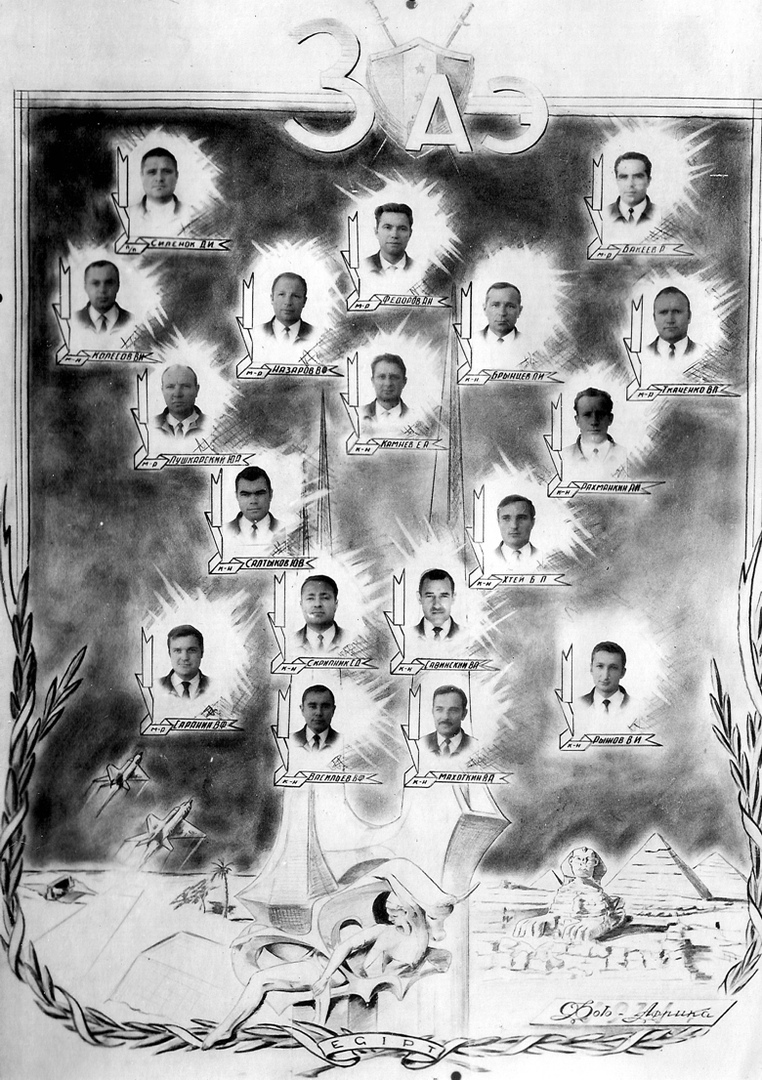
\includegraphics[scale=0.25]{Dolina_5/Nzt1_-t0RiE.jpg}
	%	\label{fig:scipion} % Unique label used for referencing the figure in-text\end{document}
	%	%\addcontentsline{toc}{figure}{Figure \ref{fig:placeholder}} % Uncomment to add the figure to the table of contents%----------------------------------------------------------------------------------------
	\caption{3-я эскадрилья 135-го ИАП. Отметим, что правильном написание фамилии ведущего четвёрки — Камнев. Никакого Ивлева нет. Журавлева тоже нет — он погиб. Звено Саранина (внизу) присутствует на виньетке, так как в конце 70-го было переведено в 3-ю эскадрилью и заканчивало «тур» в её составе.}%	CHAPTER 2
\end{figure}

Если бы Ивлев действительно существовал — он мог быть пилотом только 3-й эскадрильи из Ком-Аушим. Список её лётчиков известен — фамилии Ивлев нигде не фигурирует. При этом обстоятельства поражения «Миража», повторюсь, очень похожи на правду.

Итак. Время — приблизительно 14:38. Два русских МиГ-21 сбито. Один «Мираж» повреждён. К месту боя подходит ещё одна четвёрка 21-х и два «Миража» пары Корен-Рихтер, до этого «прятавшиеся» в радиотени. Ещё 4 «Миража» и «Фантома» ведут бой с 6 оставшимися МиГ-21.

Приблизительно в этот момент (возможно — раньше) 1-е звено выходит из боя.

Акименков:

\begin{textcitation}
	Когда звено из Ком-Авшима уже вышло из боя, к месту схватки подошло звено из Бени-Суэйфа.
\end{textcitation}

При всём уважении к Акименкову, у меня есть некоторые сомнения в том, что звено из звено Каменева вышло из боя до того, как там появилось звено Юрченко. Это просто не складывается из общей картины боя: тогда получается, что у звена Каменева было топлива где-то на 2 минуты боя. При этом у «Миражей» хватило топлива не только на бой, но и на преследование уцелевших. Не складывается что-то.

Но то, что у первого звена топливо закончилось раньше — как раз весьма закономерно: оно и взлетело на несколько минут раньше.

Косвенно, выход из боя первого звена подтверждается в книге Дани Шалома:

\begin{textcitation}
	Внезапно они [Сэла - Фишер] обнаружили два МиГа, удаляющихся из [района] боя на малой высоте. Авиам спикировал в их сторону, занял позицию для стрельбы позади одного из них, однако пилот МиГа заметил его и увернулся, резко повернув. Второй самолет был слишком далеко.
\end{textcitation}

Продолжаем.

Итак, судя по всему, звено Камнева выходит из боя — на форсаже, с большой перегрузкой, чтобы не получить ракету в спину. Звено Саранина ещё в нескольких минутах от места боя. В итоге, трое советских лётчика звена Юрченко остаются один на один с семью (а чуть позже — десятью) израильскими. И только теперь — да, действительно, численное превосходство противника становится пугающим. К тому же «Фантомы» успевают набрать достаточно скорости для маневрирования, теперь пришло их время.

Советские лётчики обескуражены тем, как разворачиваются события.

Авием Села:

\begin{textcitation}
	Они шли на нас парами, а мы дали им всем проскочить, чтобы не дать им взять нас в клещи, как они планировали. Они промчались мимо нас, пара за парой, как на параде. Мы подождали и направились за ними, зажимая их между собой. Перед нами было 16 МиГов! Я никогда не видел столько машин в одном бою. Небо было заполнено истребителями, беспорядочно маневрирующими в сумятице боя. Повсюду падали подвесные баки. Я не боялся их численного превосходства. Меня лишь страшила возможность столкновения с другим самолетом или одним из падающих баков. Я заметил, как один МиГ в двух километрах от нас начал правый вираж, чтобы зайти сзади моего ведущего. Я тоже развернулся вправо и русский пилот атаковал меня, отказавшись от преследования моего ведущего. МиГ пикировал на меня сверху, что давало ему определенное преимущество. Я резко бросил свой «Фантом» влево и мы крутились вдвоем, снижаясь, пока не достигли высоты 5000 метров. В этот момент мы были всего в 150 метрах друг от друга. 
	
	Много лет назад, еще будучи пилотом «Мистера», Авиам освоил манёвр «дай ему проскочить» Яка Нево, одного из основателей израильской школы тактики воздушного боя. Обнаружив МиГ за своей спиной, он бил по тормозам и делал «бочку», в бешеной круговерти уходя от погони. Авиам сделал это и сейчас. Как всегда, прием выручил его. МиГ проскочил вперед и Села быстро зашел ему в хвост. Русский летчик пытался оторваться на очень крутых виражах, а затем перешел в крутое пике. Противники опускались все ниже и ниже, отчаянно маневрируя и выжимая из своей машины все, на что она была способна. Штурман Авиама, Реувен Решеф, приник к приборам системы управления огнем, стремясь ни на секунду не пропустить сигнал о том, что головки наведения ракет среагировали на жар, исходящий из сопла двигателя МиГа. Наконец, на высоте двух тысяч метров и на дистанции в один километр, захват произошел и Авиам произвел пуск ракеты. С огромной скоростью «Сайдуиндер» устремился к цели и поразил ее. Раздался мощный взрыв и МиГ превратился в огненный шар, с обломками разлетавшимися во все стороны. Останки самолета падали вниз, раскручиваясь в воздухе. Поразительно, но пилот успел катапультироваться и раскачивался на стропах парашюта. 
\end{textcitation}

Как, как он насчитал 16 МиГов?!

Другое описание этого эпизода (из книги Дани Шалома):

\begin{textcitation}
	Авиам Сэла, ведомый Авигу [Бен-Нуна]: "Начался бой, а я смотрю и вижу, что Авигу попал в "сэндвич" - МиГи шли парами, а мы были в вираже. Авигу преследовал МиГи, а другие подошли к нему сзади. [по-русски это называется "слоеный пирог"?] Он попал в "сэндвич", и я предупредил его, чтоб он шел за [теми] МиГами[, что были] позади. Я сказал ему: "Не продолжай [преследование]! Пойдем за следующими МиГами". <...>
	
	...Авиам и Фишко, его оператор, оставались выше, пытаясь засечь МиГи - однако те один за другим улизнули и скрылись. Внезапно они [Сэла - Фишер] обнаружили два МиГа, удаляющихся из [района] боя на малой высоте. Авиам спикировал в их сторону, занял позицию для стрельбы позади одного из них, однако пилот МиГа заметил его и увернулся, резко повернув. Второй самолет был слишком далеко.
	
	Другой МиГ летел на него на высокой скорости. Он резко увернулся от него [видимо, А.Сэла от МиГа]. Авиам: "Русские маневрировали группами и по одному, но серьезно нам не угрожали. Они выпустили огромное количество ракет, впустую, бесцельно и бездумно. Мы с Авигу крутились там некоторое время, не сумев нацелиться [ни] на один из МиГов - каждый раз, едва мы атаковали один, сзади появлялся другой. МиГи стреляли из любых положений и ситуаций. Нельзя было поймать МиГ, не подвергая себя опасности. Вскоре мы разделились, [так как] боялись, что бой закончится для нас без единого сбитого самолета".
	
	Авиам поймал взглядом один из МиГов. Он повернул в его сторону [видимо, А.Сэла повернул в сторону МиГа-?] и два самолета выполнили серию маневров, но [ни один из них] не занял позицию для стрельбы. Этот МиГ выполнил плавный вираж и вышел в лобовую атаку. "Это моя цель, я не дам ему уйти", - пообещал себе Авигу. МиГ был уже близко и проскочил - Авиам увеличил обороты двигателей, потянул ручку управления самолетом на себя и бросил ревущий "Фантом" в жесткий маневр. Быстро [выполненный] иммельман вывел его [на позицию] выше и позади русского МиГа.
	
	"Я заметил, что один из МиГов пытается атаковать меня. Он резко отвернул, попытался поднять нос и допустил все возможные ошибки" ... "Он поддался [возможный вариант перевода - "клюнул", "купился"] на мои маневры и оказался на встречном курсе спереди и выше - идеальное для меня положение. Мы начали [крутить] виражи на высоте 15000 футов. Он продемонстрировал очень низкий уровень подготовки. После двух-трех виражей я набрал скорость, мы снизились. На высоте 2000 футов я достиг подходящей дистанции и произвел пуск ракеты. Ракета пошла, достигла цели, произвела огромный взрыв, и я уже начал хрипеть [от восторга]. И тут из этой большой [вспышки] огня вылетел МиГ - совершенно целый!
	
	Я произвел пуск второй ракеты - но прежде, чем она попала, МиГ развалился на части. Очевидно, что первая ракета поразила его, но у меня не хватило терпения дождаться результатов".
	
	Первая ракета... взорвала русский МиГ и развалила его на части. Для второй ракеты уже не было цели, и она скрылась среди обломков.
	
	Сэла: "Пилот выпрыгнул. Я резко повернул и проверил, что позади меня нет никаких самолетов".
\end{textcitation}

Две тысячи метров или футов? Не знаю, в обоих случаях так в источнике, а я больше доверяю Дани Шалому в этом вопросе.

Авиам Села сбил Яковлева — четвёртого номера невезучего звена Юрченко. Он погиб при приземлении.

Акименков:

\begin{textcitation}
	Лётчик благополучно катапультируется. Но неблагополучно приземляется. Воздушный поток срывает незастёгнутый защитный шлём. Приземление происходит среди скал и камней. Подворачивается нога. Удар головой о камень. Смерть
\end{textcitation}

В то время, как Села воюет с МиГами, его товарищи пытаются преследовать выходящую из боя первую пару звена Юрченко — собственно Юрченко и Макара.

Юрченко пытается на форсаже уйти в сторону своего аэродрома. На малой высоте и максимальной скорости. Вообще, пытаться уйти от «Фантома» по прямой на 21-м — специфическая разновидность суицида. «Фантом» быстрее, а главное — имеет ракеты с полуактивной ГСН. Правда, на фоне земли РЛС «Фантома» не видит цель — а значит, не может захватить её.

МиГ Юрченко летел низко, на высоте около 50 метров. Против любых других лётчиков этого было бы достаточно. Но на его беду, человек, сидевший в кабине «Фантома», умел летать действительно низко. А в его задней кабине сидел один из лучших операторов РЛС «Фантома» на этом берегу Атлантического океана.

\begin{textcitation}
	МиГ был в полутора километрах впереди нас. Меня беспокоило только одно: как бы пилот 'Миража' не сбил МиГ раньше меня. У него были израильские ракеты 'Шафрир', а у меня американские 'Сайдуиндеры'. Наконец, я смог произвести пуск ракеты, но из-за чрезвычайно высокой скорости МиГа, захват был сделан на самом пределе. Ракета поразила цель и взорвалась. Но, казалось, повреждения были недостаточны, т.к. МиГ продолжал лететь, даже не сбавляя скорость. Мой штурман посоветовал использовать радиолокационную ракету 'Спарроу'. Я сам даже не подумал о ней, т.к. тот тип, что был у нас, был устаревшим и не предполагался к использованию на столь малой высоте. В это время мы приблизились к долине Нила и оказались несколько выше. Сейчас наши шансы стали чуть лучше и я знал, что мой штурман отлично владеет техникой наведения с помощью радара. Он захватил цель и я произвел пуск. 'Спарроу' настигла МиГ и он взорвался. Я уверен, что летчик погиб, т.к. было слишком низко для успешного катапультирования.
\end{textcitation}

И описание из книги Дани Шалома:

\begin{textcitation}
	Медленно и поэтапно начали русские самолеты выходить из боя. <...> Авигу на "Фантоме" [с бортовым номером] 105 издали заметил блестящий МиГ, уходящий из района. Позади него и сбоку были два "Миража", оставшиеся от четверки 117 [эскадрильи] - он [кто?] [еще] не заметил их в этот момент.
	
	Это были Иегуда Корен и Коби Рихтер. В русском самолете был Камнев, ведущий одного из звеньев, взлетевших с Ком-Аушим. Он предпочел улизнуть. Иегуда и Коби заметили удаляющийся МиГ и преследовали его на высокой скорости. "Мы увидели один самолет, болтавшийся в районе боя. Это было на высоте 1000-2000 футов над поверхностью". Коби поспешил выпустить ракету "Шафрир 2" - слишком далеко, ракета устремилась за МиГом, но не настигла его и упала на землю. Иегуда занял позицию позади русского МиГа, был готов стрелять, поднял "ложечку", закрывающую кнопку [пуска] ракет, нажал - и никакой реакции! Ракет под крыльями его "Миража" не было. Когда он сбрасывал подвесные баки, набирая высоту при вступлении в бой, две его ракеты "Шафрир 2" также отцепились и упали на землю.
	
	Расстроившись, он попытался приблизиться к МиГу на дистанцию [стрельбы из] пушек, когда над ним пролетела ракета "Спэрроу", белая и огромная, за которой тянулся густой белый дым.
	
	"Что происходит?" - он устремил взгляд назад.
	
	Сразу следом за ракетой послышался грохот "Фантома", который выпустил ее, и пролетел мимо на высокой скорости. Это был самолет Авигу и Леви, преследовавший ускользающий МиГ Камнева. Авигу, у которого [в этот момент] больше, чем когда либо, [проявился дух] состязательности, опасался, что Корен опередит его и собьет этот МиГ. Он заторопился.
	
	"Мы летели [выстроившись] линией, примерно в тысяче метров от самолета, несущегося на малой высоте к Нилу. На снижении [сходе с холмов???] я произвел по нему пуск [ракеты] "Дэкер" - которая из-за высокой скорости [цели] и [большой] дистанции - повредила его очень незначительно. Он продолжал лететь, оставляя за собой шлейф топлива".
	
	Авигу был непреклонен в стремлении сбить этот МиГ. Они летели на предельно малой высоте. Он удивился той скорости, с которой летел этот МиГ - по разведданным, имевшимся в ВВС Израиля, МиГи не могли развивать такую скорость на малой высоте. Но это был МиГ новой и незнакомой модификации.
	
	Шауль Леви, высококлассный оператор систем вооружения, умел понимать изображение на РЛС даже на фоне помех от поверхности.
	
	"Нормально, - сказал Шауль Авигу, - Я захватываю его [радаром]!"
	
	"Кто на самом деле сделал всю работу, так это мой оператор, Шауль Леви, - рассказывает Авигу, - Это было незаурядно, так как нужен высокий уровень мастерства, чтобы различить отраженный сигнал цели на такой малой высоте. Это было на снижении, а МиГи не держали действительно малую высоту, [??] было еще несколько десятков метров до поверхности. Но Шауль смог захватить [его радаром]".
	
	Леви смотрел на экран РЛС и на фоне отраженных от поверхности сигналов различил МиГ, движущийся по экрану.
	
	"Жди. Жди. Жди. Жди, - сказал он Авигу. - Сейчас - пуск!»
	
	Все произошло быстро. На РЛС появилась индикация захвата. Авигу нажал на гашетку. Ракета сошла с подфюзеляжного пилона, повернула в направлении МиГа и врезалась в него с большой силой. МиГ взорвался и развалился в воздухе.
	
	У Камнева, ведущего звена, которое первым вступило в бой, не было никакой возможности покинуть [машину].
	
	"Ракета уничтожила его очень низко на скорости близкой к скорости звука... Это был, очевидно, модернизированный МиГ, обладавший возможностью летать на скорости звука на такой высоте", - вспоминает Авигу.
	
	Ури Гиль слышал переговоры [по ходу] этого боя и видел краем глаза[, как] Авигу, сидел на хвосте у ["]своего["] МиГа внизу, почти на высоте [верхушек] деревьев, и сбил его. Коби Рихтер, маневрировавший вместе с [Иегудой] Кореном позади МиГа, был расстроен. Не [их] "Миражи" сбили этот МиГ, а сосед с [базы] Рамат-Давид: он [И.Корен] видел [ракету] "Спэрроу", оставившую длинный белый шлейф, и попадание в МиГ и описал позднее, как этот МиГ превратился в "космическую пыль".
\end{textcitation}

Здесь у Дани ошибка — это был не Каменев, а Юрченко — единственный погибший, не сумевший выпрыгнуть.

Вообще, в чем-то очень забавно получается. Ни один из известных мне русскоязычных источников не сумел описать обстоятельства его гибели правильно — включая тех, кто был непосредственно на месте событий. Это ещё раз показывает проверенный годами факт.

Итого. Сбито 4 МиГ-21. В районе боя — 2«Фантома», 6«Миражей» и на всю эту толпу — одинокий МиГ капитана Макары, последний оставшийся из разгромленной четвёрки Юрченко. Удивительно — но ему, единственному, удалось уцелеть!

По моему мнению, МиГ капитана Макары — и есть тот самый, таинственный пятый сбитый советский самолёт. С этим самым пятым вот какая история.

Сразу после окончания боя, израильтяне записали себе четыре (!) победы. То есть те, в которых они были полностью уверены. На пятую претендовали сразу два лётчика, но подтвердить её данными радиоперехвата было сложно.

Засчитали её только в 73-м году, после Войны Судного дня.

В реальности, капитан Макара сумел сесть на повреждённом самолёте в Ком-Аушим. Вот как это было:

Акименков:

\begin{textcitation}
	А ведомого на «кадушке» пытается достать своей пушкой настойчивый «Мираж», превращая его стабилизатор в решето. Лётчик уходит на вертикаль. Выполняет одну «мёртвую петлю», вторую и сваливается в её верхней точке в штопор. Отпускает ручку управления, вращение прекращается и мимо него проходит вниз, как ни в чем не бывало, уже упомянутый «Мираж». У него меньше нагрузка на крыло и он обходится без штопора, но оказывается под МиГом.
	
	Наш лётчик подтягивает нос самолёта, чтобы стрельнуть из пушки и снова вращается в штопоре. Позже они летят некоторое время на параллельных курсах. Причем наш летит домой. У него топливо на исходе.
	
	Прошли траверз засадного аэродрома Катамия. Наш лётчик не может сесть там, поскольку его беспомощностью на посадке тут же воспользуется противник. Впереди замаячили контуры аэродрома Каир-Вест, очерченные позициями пулемётов, пушек и ракет разных калибров в несколько ярусов. Израильтянин осознаёт глупость происходящего и разворачивается на обратный курс.
\end{textcitation}
Рыболовлев:

\begin{textcitation}
	Из звена Юрченко произвел посадку Макара, и то не на своем аэродроме, из-за повреждения системы управления. Макара в перископ увидел как заходит сзади для атаки Мираж, резко взял ручку на себя и с углом кабрирования 85 градусов пошел вверх. Набор высоты продолжался до потери скорости и сваливания самолета. Самолет через крыло развернулся носом вниз. Все происходило при включенном форсаже. Мираж на вертикали отстал, но когда самолет Макара совершал разгон, устремился за ним. Набрав скорость (более 1000 км/час, точно не помню) Макара вновь выполнил резкий набор высоты с последующим пикированием, противник или отказался от преследования или потерял цель. Макара выровнял самолет в горизонтальный полет на высоте 600 - 800 метров, и справа (может слева, не помню) очень близко увидел приближающийся Фантом. Резко довернул самолет в сторону противника. Однако летчик Фантома успел поразить самолет Макара очередью из пушки. Очередь (8 или 10 снарядов) прошла по килю и форсажной камере. Из-за очень близкого расстояния снаряды не взорвались (не успели взвестись), однако управление было повреждено (кажется, затруднено было управление по высоте).
\end{textcitation}

\begin{textcitation}
	Из звена Юрченко произвел посадку Макара, и то не на своем аэродроме, из-за повреждения системы управления. Макара в перископ увидел как заходит сзади для атаки Мираж, резко взял ручку на себя и с углом кабрирования 85 градусов пошел вверх. Набор высоты продолжался до потери скорости и сваливания самолета. Самолет через крыло развернулся носом вниз. Все происходило при включенном форсаже. Мираж на вертикали отстал, но когда самолет Макара совершал разгон, устремился за ним. Набрав скорость (более 1000 км/час, точно не помню) Макара вновь выполнил резкий набор высоты с последующим пикированием, противник или отказался от преследования или потерял цель. Макара выровнял самолет в горизонтальный полет на высоте 600 - 800 метров, и справа (может слева, не помню) очень близко увидел приближающийся Фантом. Резко довернул самолет в сторону противника. Однако летчик Фантома успел поразить самолет Макара очередью из пушки. Очередь (8 или 10 снарядов) прошла по килю и форсажной камере. Из-за очень близкого расстояния снаряды не взорвались (не успели взвестись), однако управление было повреждено (кажется, затруднено было управление по высоте).
\end{textcitation}

Здесь снова ошибка — это не Журавлёв, это именно Макара. Журавлёва сбил Села несколькими минутами раньше. Отметим — падения самолёта израильтяне не видели, и справедливо НЕ засчитали его на свой счёт в тот момент.

Примерно в этот момент происходит достаточно комичная ситуация. Исраэль Бахарав, вторая пара из Рефидим, пытается войти в бой. Проблема в том, что они прибывают поздно и не успевают к основному действу.

В то же время на месте боя появляется третья четвётка советских истребителей (звено Саранина), на подходе — ещё два звена с Бени-Суэф и Ком-Аушим. Каким-то чудом советские лётчики и израильтяне ухитряются пройти мимо друг друга, не заметив противника. Бахарав рисковал столкнуться с двенадцатью советским лётчиками. Но… скажем так. Этот человек был легендой даже внутри израильских ВВС — из-за умения стрелять из любых положений и с любым упреждением. И попадать в цель. Он прошел «Мокед», и к июлю 70го на его счету было шесть египетских МиГ-21. Через три года, без ракет, с неисправным двигателем, и с семью (!) оставшимися снарядами он будет как безумный носиться над Дельтой в поисках египетских самолётов.

Четверо, двенадцать, или двадцать — будущий король израильских IT-стартапов и будущий зам главкома ВВС — не совсем те люди, с которыми стоило встречаться в тот день.

Возвращаемся к Римон-20.

Капитан Макара совершил настоящее маленькое чудо. На него охотились люди, на счету которых было 22 сбитых самолёта. Легенды. Йифтах Спектор, Авраам Салмон, Коби Рихтер, Эхуда Корен — на их счету было 50 сбитых арабских самолётов (подтверждается что-то около 40-45). Он ушел от нескольких ракет, получил очередь из пушек «Миража» (тут сложно понять, чьей — вероятно, Спектора). И сумел вернуться домой.

В некоторых советских и большинстве израильских источниках его считают сбитым (и даже погибшим) — это не соответствует действительности.

Тот трагический для советских ВВС день завершился.

Четыре МиГ-21 догорали кострами в Дельте, как памятник самоуверенности людей, приславших их в Египет. Трое из четырёх советских лётчиков погибли. Их жизни — на совести генерала Дольникова, героя Великой Отечественной войны и просто отличного офицера. Его беда и трагедия — в том, что опыт, которым он обладал, безнадёжно устарел. Человек на другой стороне, Мордехай Ход, не прошёл и десятой доли испытаний, выпавших Дольникову. Просто бывший командир эскадрильи «Мустангов», непрерывно воевавший последние полтора десятка лет, был лучше. Как командир, как организатор. И люди, которые были там — они прошли огонь и воду, а медные трубы им пока не грозили. Когда советские лётчики готовились к большой войне — израильские пытались как-то выжить уже сейчас. Когда капитан Яковлев учился перехватывать неманеврирующую мишень в Марах, Ашер Снир штурмовал египетские аэродромы на высотном перехватчике с парой бомб. Когда капитан Сыркин учился вести воздушный бой в Тирасполе, Итамар Нойнер горел над Синаем, пытаясь выиграть лишние пару километров между жизнью и смертью. А Амос Амир прыгал из обреченного «Миража» с отказавшим двигателем над Хатцором.

Когда Григорий Устинович Дольников стал зам главкома ВВС СССР, Ифтах Спектор уже похоронил половину своих однокурсников.

Не бывает побед без потерь. Любой опыт в таких делах оплачивается кровью. И каждый из израильских пилотов знал слишком много хороших друзей, которые взлетели и не вернулись. Дан Энгель. Дан Сигри. Шломо Бен-Ор. Яир Нейман. Давид Барух. Беньямин Ромах. Шломо Вейнтрауб. И дюжины других.

Израильский опыт, обеспечивший им победу, был уже оплачен. Наш — ещё нет.

Потому что израильтяне прошли все возможные ошибки, и сотворили почти невозможное, штурмуя на высотных перехватчиках египетские аэродромы в 67м. Каждый десятый лётчик, участвовавший в «Мокеде», остался в Египте.

Штурмуя иорданские укрепления в Иерусалиме и сирийские «фестунги» на Тель-Фахр на учебных «Фугах».

Нет позора в том, чтобы проиграть таким людям. Советские лётчики отважно сражались и погибли героями. То поражение дало СССР больше, чем дала бы любая победа. Понимание того, что подготовка советских лётчиков несовершенна — дорогого стоила. Благодаря египетскому опыту, в СССР пересмотрели подход к подготовке лётчиков-истребителей. Точно так-же, как американцы после первых проблем Вьетнама разрабатывали новые подходы к обучению пилотов. Они основывались на опыте, которые был прекрасно понятен оппонентам советских пилотов на Ближнем Востоке.

\section{Выводы:}

Главной причиной поражения стала не воздушная засада, не фактор внезапности и даже не действия «Масреги». Главной причиной стала именно пресловутая «разница в подготовке и опыте».

К чести советских лётчиков в Египте, они быстро поняли, что к чему, и оперативно перестроили подход к обучению. Не исключено, что ещё один или два боя — и советские лётчики смогли бы создать массу проблем. Всё-же в Египте был весь цвет строевой истребительной авиации великой красной сверхдержавы. Олег Григорьевич Цой и Александр Вениаминович Акименков стали в будущем заслуженными лётчиками-испытателями. Григорий Устинович Дольников, командир авиагруппы — стал заместителем Главкома ВВС СССР.

Тот единственный бой над Египтом дал бесценный опыт и понимание собственных ошибок и огрехов. Этот опыт был оплачен кровью — впрочем, знаменитый американский Топ Ган и менее известные программы переподготовки пилотов ВВС США тоже были оплачены жизнями десятков пилотов ВВС и Флота во Вьетнаме.

Что самое удивительное — сами советские пилоты, даже самые уважаемые, так и не смогли понять, что (и почему) тогда произошло.

Акименков:

\begin{textcitation}
	Все последующие дни до перемирия мы пытались вызвать противника на ответный бой. Но рыцарские дуэли в Израиле не в почете. Элитная 101-я эскадрилья, основной контингент которой состоял из наёмников, пропивала призовые деньги на тыловых базах и наши проблемы её не интересовали.
\end{textcitation}

И снова — наёмники, американцы, вьетнамский опыт. Складывается ощущение, что они нарисовали себе в голове картинку (или им её нарисовали), которой было проще всего придерживаться. 101-я — одна из трёх «строевых» эскадрилий «Миражей». Самое смешное, что её пилоты практически не участвовали в том бою.

\begin{textcitation}
	Смысл сказанного состоял в том, что снимаются все запреты и ограничения на пилотаж и боевое маневрирование. Воздушную подготовку мы должны были начать с чистого листа и руководствоваться в ней своим здравым смыслом, а не чужой совестью. Генерал призвал нас верить собственным инстинктам и интуиции, а сам обязался верить в нашу общую удачу.
\end{textcitation}

По большому счету, только тогда для многих советских пилотов открылись совершенно новые горизонты.

Сами израильтяне отозвались о советских пилотах смешанно, назвав их хорошими пилотажниками, но очень неопытными бойцами. Плёнки и прочие свидетельства боя были немедленно изъяты, пилотам засчитали 4 сбитых египетских самолёта.

В 1973-м году по данным разведки, Спектору и Салмону засчитали тот самый пятый сбитый. Причина такого долгого промежутка не вполне понятна. Есть гипотеза, что МиГ-21 капитана Макары был каннибализирован.

\begin{figure}[h!tb] 
	\centering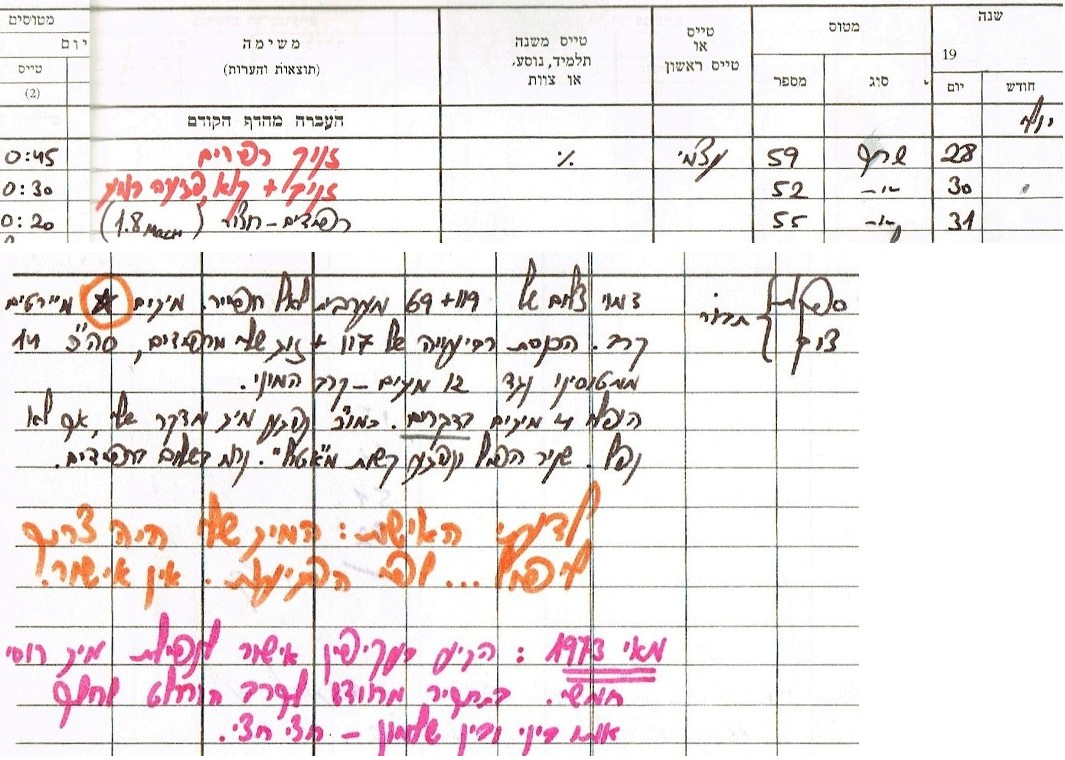
\includegraphics[scale=0.25]{Dolina_5/AuXZifeT9e0.jpg}
	%	\label{fig:scipion} % Unique label used for referencing the figure in-text\end{document}
	%	%\addcontentsline{toc}{figure}{Figure \ref{fig:placeholder}} % Uncomment to add the figure to the table of contents%----------------------------------------------------------------------------------------
	\caption{Лётная книжка Спектора (запись о сбитом самолёте — внизу, фиолетовым).}%	CHAPTER 2
\end{figure}

\begin{figure}[h!tb] 
	\centering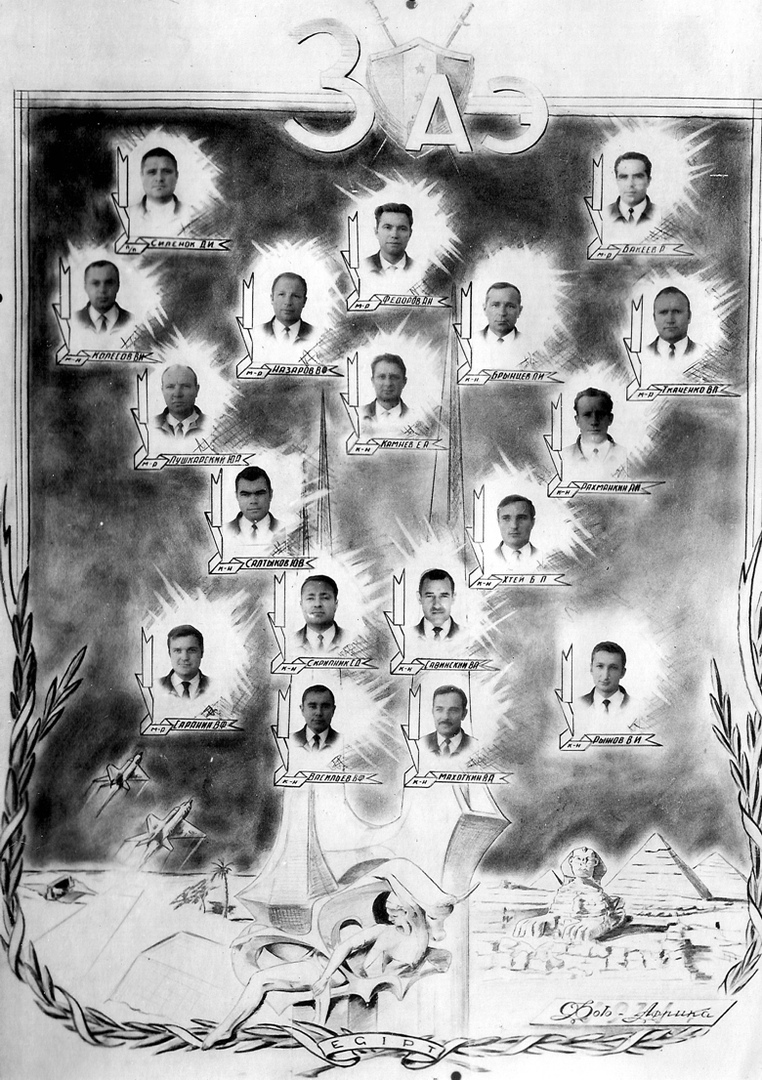
\includegraphics[scale=0.25]{Dolina_5/Nzt1_-t0RiE.jpg}
	%	\label{fig:scipion} % Unique label used for referencing the figure in-text\end{document}
	%	%\addcontentsline{toc}{figure}{Figure \ref{fig:placeholder}} % Uncomment to add the figure to the table of contents%----------------------------------------------------------------------------------------
	\caption{сертификат об одержанной победе. Отмечаем — он 1973 года}%	CHAPTER 2
\end{figure}

Закончить я хотел бы продолжением той фразы, которой начинал этот цикл, сказанной Дольниковым:

\begin{textcitation}
	Эти несколько фраз определили сразу и суть задачи, и способ её решения. Только полная свобода индивидуального и коллективного творчества, в том числе - творчества подсознательного, могла привести к победе, поскольку никто не знал даже общих подходов к ней.
\end{textcitation}


\section{Список источников.}

Книги:

\begin{enumerate}
	
	
	\item  «Оспреевская» серия Шломо Алони (Israeli F-4 Phantom II Aces и Israeli Mirage Aces). Оттуда-же взято множество фотографий. (англ.)
	
	\item  «Призраки над Каиром» Дани Шалома (ивр.).
	
	\item  Б.В. Абрамов, «Голубое небо Египта»
	
	\item  «Тогда в Египте», глава «Дан приказ ему … в Египет», написанная Ельчаниновым
	
	\item  «Israel's Best Defense: The First Full Story of the Israeli Air Force» Элиэзер Коэн (англ.)
	
	\item  «Loud and Clear» Ифтах Спектор (англ.)
	
	\item  «От имени Неба» Авирам Баркаи (ивр.)
	
	\item  «Arab MiGs vol.5» Том Купер и Дэвид Николле (англ.)
\end{enumerate}
Сайты:
\begin{enumerate}
	
	
	\item  http://hubara-rus.ru, сайт организации ветеранов войны в Египте. Множество фотографий взято оттуда
	
	\item  http://www.sky-high.co.il — «Махиа Шхаким», сайт Амира Сегева и Авиноама Мисникова (ивр.). Взяты в первую очередь фотографии.
\end{enumerate}
Форумы:
\begin{enumerate}
	
	\item  http://forums.airbase.ru/2007/07/t25657\_32--vojna-na-istoschenie-1967-1970.html — дискуссия на форуме «Авиабазы», там 32 страницы пошагового разбора.
	
	\item  http://forums.airforce.ru/holodnaya-voina/132-boi-v-egipte-1970-a-2/ — форум сайта Airforce.ru.
	
	\item  https://www.fresh.co.il/vBulletin/showthread.php?t=584112 — история службы Ифтаха Спектора (ивр.)
\end{enumerate}
Статьи:
\begin{enumerate}
	
	\item  https://www.makorrishon.co.il/nrg/online/1/ART/969/882.html — история «Гречкоим» (ивр.)
	
	\item  ЖЖ https://morelas.livejournal.com/1943.html — очень подробное собрание воспоминаний участников, с переводами
	
	\item  http://navoine.info/isr-eg-1970.html — огромная статья Наума Шубаева, перевод главы из «Признаков над Каиром» Дани Шалома, за что ему (Науму) огромное спасибо
	
	\item  http://old.hubara-rus.ru/135iap.html — фотографии пилотов
	
	\item  http://nvo.ng.ru/notes/2005-10-07/8\_vyvod.html — рассказ Сыркина
\end{enumerate}
И многое другое, о чем я забыл)
